%\documentclass[unicode]{scutthesis} % 草稿封面,硕士则添加选项master,博士则去掉
\documentclass[unicode,pdfcover,review]{scutthesis} %   % 送审版
%\documentclass[unicode,pdfcover]{scutthesis} %   % 最终版
\usepackage{color,array,longtable,graphicx,multirow,makecell,hhline} % 增添makecell,hhline宏包对三线表进行定制 revised by CYX
\usepackage{placeins}
\usepackage{changes} % 说明了本版本主要修改了什么 revised by CYX
% 物理单位设定 by CYX
\usepackage[italic,defaultmathsizes]{mathastext}
\usepackage{siunitx}
\sisetup{input-digits = 0123456789\pi}
\sisetup{per-mode = symbol}%
\DeclareSIUnit \vHardness {Hv} % 维氏硬度Hv
\DeclareSIUnit \dBA {dBA} % 动态范围
\DeclareSIUnit \mT {mT} % 特斯拉
\DeclareSIUnit \pt {pt} % pt
\newcommand{\qtyRange}[3]{\qtyrange[range-units=single,range-phrase=-]{#1}{#2}{#3}} % 单位范围
\newcommand{\numRange}[2]{\numrange[range-phrase=-]{#1}{#2}}	% 数字范围
%%%%%%%%%%%%%%%%%%%%%%%%%%%%%%%%%%%%%%%%%%%%%%%%%%%%%%%%%%%%%%%%%%%%%%%%%%%%%%%%%%——by MCH
%编译范围
%\includeonly{content/chapter3.tex}
%参考文献设置
\usepackage[backend=biber,style=gb7714-2015,gbalign=gb7714-2015,gbpub=false,gbnamefmt = lowercase]{biblatex}
\setlength{\bibitemsep}{0ex} % 设置参考文献条目间距离 revised by CYX
\renewcommand{\bibsetup}{
	\interlinepenalty=1000\relax
	\widowpenalty=1000\relax
	\clubpenalty=1000\relax
	\raggedbottom
} % 参考文献条目跨页设置,避免太大空行 by CYX
\addbibresource[location=local]{MyLibrary.bib} % 如果在其他盘,改为相对路径。比如F盘,改为:F/MyLibrary.bib
%页眉页脚设置
\usepackage{fancyhdr}
\usepackage{listings}
\usepackage{xunicode}
\renewcommand{\lstlistingname}{列表}
\pagestyle{fancy}
\fancyfoot[C]{\headfont\thepage}

\renewcommand{\chaptermark}[1]{\markboth{\chaptername\ #1}{}}
\renewcommand{\sectionmark}[1]{\markright{\thesection\ #1}}
\fancyhead[RE]{}
\fancyhead[RO]{}
\fancyhead[LE]{}
\fancyhead[LO]{}
\fancyhead[CO]{\headfont{\leftmark}}
\fancyhead[CE]{\headfont{华南理工大学博士学位论文}}% 
\renewcommand{\headrulewidth}{1.5pt}
\renewcommand{\footrulewidth}{0pt}
%%%%%%%%%%%%%%%%%%%%%%%%%%%%%%%%%%%%%%%%%%%%%%%%%%%%%%%%%%%%%%%%%%%%%%%%%%%%%%%%%%
\usepackage[unicode=true,bookmarks=true,bookmarksnumbered=true,bookmarksopen=false,breaklinks=false,pdfborder={0 0 1},backref=false,colorlinks=true]{hyperref}
\hypersetup{pdftitle={论文},
	pdfauthor={崔延鑫},
	pdfsubject={华南理工大学博士学位论文},
	pdfkeywords={A;B},
	linkcolor=black, anchorcolor=black, citecolor=black, filecolor=black, menucolor=black, urlcolor=black, pdfstartview=FitH}% 黑白,提交版
%%	linkcolor=blue, anchorcolor=black, citecolor=red, filecolor=magenta, menucolor=red, urlcolor=magenta, pdfstartview=FitH}% 彩色

\makeatletter
%%%%%%%%%%%%%%%%%%%%%%%%%%%%%% LyX specific LaTeX commands.
\providecommand{\LyX}{\texorpdfstring%
	{L\kern-.1667em\lower.25em\hbox{Y}\kern-.125emX\@}
	{LyX}}
%% Because html converters don't know tabularnewline
\providecommand{\tabularnewline}{\\}
\makeatother
\begin{document}
	%%%%%%%%%%%%%草稿封面设置%%%%%%%%%%%%%	
	\title{LaTeX模版说明}	
	\author{崔延鑫}	
	\supervisor{指导教师:石永华\ 教授}	
	\institute{华南理工大学}	
	\date{}
	%%%%%%%%%%%%%%%%%%%%%%%%%%%%%%%%%%%%%
	\maketitle	
	\frontmatter	%此后为罗马数字页码,页面类型为plain
	\chapter{摘\texorpdfstring{\quad}{}要}
	本模板由Shun Xu\cite{_}、yecfly\cite{_a}\added{以及mengchaoheng\cite{_mengChaoHeng}}的模板修改而来,适合于华南理工大学硕/博士毕业论文。
	既然已经入坑LaTeX,就不推荐使用LYX,但本模板在修改祖传代码过程中仅对修改部分进行更新,其余部分仍保留源代码。另外参考文献管理软件推荐使用zotero,这也是本模板使用的软件。
	本模板最主要的改动是参考文献使用biber,而不是原来的bibtex,因此不再需要.bst文件。
	\added{本模版更新了双盲评审选项,符合2022年最新的格式要求,将公式字体变更为Times New Roman等,具体细节见正文。}

\keywordsCN{\LaTeX{};论文}

\chapter{Abstract}
	

\keywordsEN{\LaTeX{}; Paper} % 中英文摘要
	%%%%%%%%%%%%%%%%%%%%%%%%%%%%%%%%%%%%%%%%%%%%%%%%
	% 目录、表格目录、插图目录这几个字本身的大纲级别是一级的,即和章名有相同的字号字体。目录表的内容通过titletoc宏包在。cls文件设置了。
	\tableofcontents	%目录
	%\listoftables	%表格目录(可选)
	%\listoffigures	%插图目录(可选)
	%%%%%%%%%%%%%%%%%%%%%%%%%%%%%%%%%%%%%%%%%%%%%%%%%
	%\include{symbols}	% 符号对照表(可选)
	%\include{abbreviation} 	% 缩略词	
	
	\mainmatter %此后为阿拉伯数字页码
	
    %%%%%%%%%%%%%%%%%%%%%%%%%%%%%%%%%%%%%%%%%%%%%%页眉页脚设置 ——by MCH 
    \fancypagestyle{plain}{
    	\pagestyle{fancy}
    }	% 每章的第一页会默认使用plain,没有页眉。通过重定义plain为fancy解决
    \pagestyle{fancy}	%设置页眉页脚为fancy
    %%%%%%%%%%%%%%%%%%%%%%%%%%%%%%%%%%%%%%%%%%%%%%分章节,结合导言区的\includeonly命令可仅编译部分章节,编译时不用切换界面,直接在相应章节编译即可。
	\chapter{绪论}
%
\section{研究背景和意义}
\subsection{研究背景和意义}
%
关于\LaTeX{}以及基于\LaTeX{}写作的好处不再赘述。\LaTeX{}的入门资料推荐文献\parencite{_b}以及文献\parencite{_c}。

这里主要是想推荐一种“学术生态”,即利用各种工具展开科研工作,以达到事半功倍的效果。需要用到以下软件:
\begin{enumerate}
	\item 	参考文献管理软件zotero\cite{_f}。很多人使用过endnote,但其实zotero也非常强大,强烈推荐。可到b站观看Struggle with Me出品的视频教程\cite{_e}入门。\replaced{最新的zotero已支持软件内部PDF阅读。}{zotero不自带pdf阅读器,使用Adobe Acrobat pro DC即可。
				在Adobe中点击文件->属性->位置,即可打开文件所在位置,故亦不推荐更改zotero的文件系统。}
	\item	可截图获取文献中公式的软件mathpix\cite{_d}。在阅读别人的论文时,很可能需要把文章中的公式抄下来放到自己的笔记中,方便以后组会报告甚至论文中使用,这时使用mathpix可直接截图获取\LaTeX{}源码,非常方便。该软件普通邮箱注册可每月50次免费,学校邮箱可100次,若信用卡注册可1000次。	
	\item	\replaced{VS Code}{TeXstudio},相当于IDE。本模板是基于\replaced{VS Code}{TeXstudio2020}进行的,关于该软件的使用(快捷键等)可另行查找资料。\deleted{编译时可以使用该软件,也可以运行文件目录的all.bat。TeXstudio的设置见第二章。}
\end{enumerate}

\added{本文总体结构以及前三章均继承了前辈们的框架与内容,本人所做修改均标注为蓝色,第四章为本人撰写,故未作颜色标记。}本文的章节安排如下:

第一章,绪论。

第二章,模板简介。主要介绍各文件的内容。

第三章,常用环境。介绍论文写作中常用的环境,包括:图、表、公式、定理。基本涵盖了常用的命令。

\added{第四章,本人对前辈们的模版的修改之处,包括:双盲评审、图、公式、参考文献、标题等。}



%第一章
	\chapter{模板简介}
%
与很多外文杂志社不同,大部分中文期刊都不提供\LaTeX{}模板给投稿者使用,也很少有学校给学生提供官方的毕业论文模板。目前github上的大部分模板都是由学生发起的非官方模板。在此感谢Shun Xu以及yecfly\added{、mengchaoheng}等人的工作,他们的无私贡献使得华南理工大学硕博士毕业论文也可以使用\LaTeX{}撰写。

本模板是直接修改前人的模板得到的,更详细的介绍可到\parencite{_,_a}下载。本章仅从用户的角度简要介绍模板的使用,而尽量避免涉及\LaTeX{}的模板制作细节(实际上是因为本人也不会)。正如我们使用手机并不需要了解麦克斯韦方程组,使用\LaTeX{}写作也无需了解模板是如何制作的。

\LaTeX{}的源代码保存在后缀名为.tex的文件中。当编写长篇文档时,例如当编写书籍、毕业论文时,单个源文件会使修改、校对变得十分困
难。将源文件分割成若干个文件,例如将每章内容单独写在一个文件中,会大大简化修改和校对
的工作。为方便,本文将scutthesis.tex文件称为主文件,而将abstract.tex、chapter0x.tex、conclusion.tex等文件称为章节文件。

值得注意的时,要每次编译时都更新参考文献著录,TeXstudio软件的选项->设置中的构建并查看、编译器需要设置成如图\ref{TeXstudio}所示。此时只需在任意一个文件中点击构建并查看按钮即可编译文档。每次编译都更新参考文献会使得编译时间很长。
\begin{figure}[htbp]
	\centering
	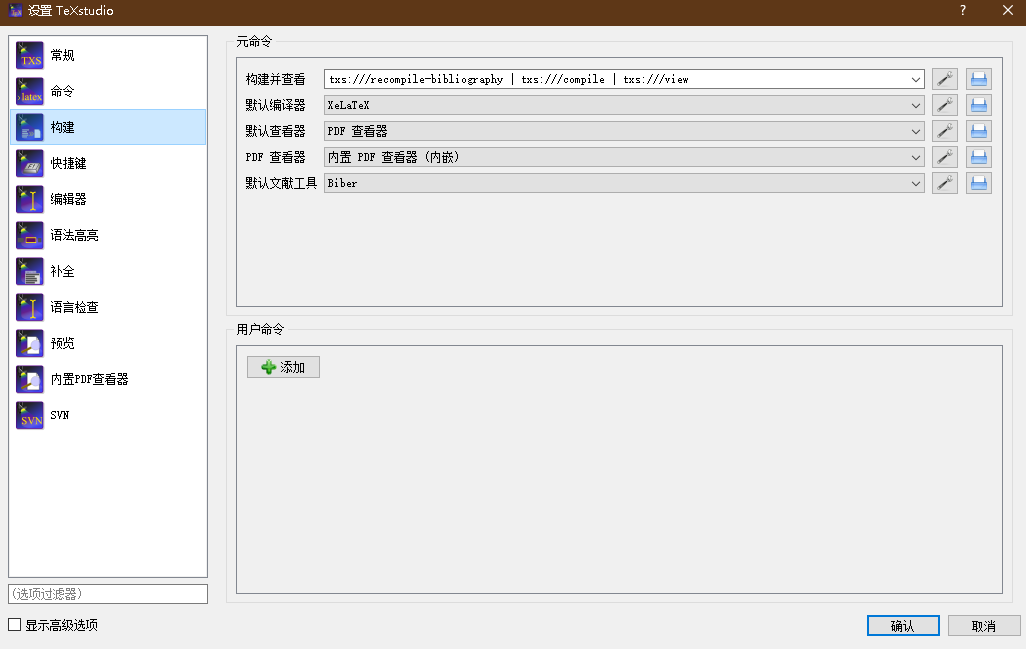
\includegraphics[scale=0.55]{Fig/TeXstudio.png}
	\caption{\label{TeXstudio}TeXstudio环境}
\end{figure}

\section{主文件}
scutthesis.tex文件相当于主函数,调用各章的内容。\LaTeX{}源代码以一个\textbackslash{}documentclass 命令作为开头,它指定了文档使用的文档类。文档类规定了\LaTeX{}源代码所要生成的文档的性质——普通文章、书籍、演示文稿、个人简
历等等。
\begin{lstlisting}
\documentclass[⟨options⟩]{⟨class-name⟩}
\end{lstlisting}
其中class-name为文档类的名称,如\LaTeX{}提供的article, book, report,可在其基础上派
生的一些文档类或者有其它功能的一些文档类。\LaTeX{}提供的基础文档类见文献\parencite{_c}。还可以自定义文档类,如华南理工大学硕博士论文文档类scutthesis,其实现保存在后缀名为.cls的文件中。可选参数options 为文档类指定选项。


document环境当中的内容是文档正文:
\begin{lstlisting}
\begin{document}
正文内容
\end{document}
\end{lstlisting}
正文中包含各章节内容:
\begin{lstlisting}
\chapter{摘\texorpdfstring{\quad}{}要}
	本模板由Shun Xu\cite{_}、yecfly\cite{_a}\added{以及mengchaoheng\cite{_mengChaoHeng}}的模板修改而来,适合于华南理工大学硕/博士毕业论文。
	既然已经入坑LaTeX,就不推荐使用LYX,但本模板在修改祖传代码过程中仅对修改部分进行更新,其余部分仍保留源代码。另外参考文献管理软件推荐使用zotero,这也是本模板使用的软件。
	本模板最主要的改动是参考文献使用biber,而不是原来的bibtex,因此不再需要.bst文件。
	\added{本模版更新了双盲评审选项,符合2022年最新的格式要求,将公式字体变更为Times New Roman等,具体细节见正文。}

\keywordsCN{\LaTeX{};论文}

\chapter{Abstract}
	

\keywordsEN{\LaTeX{}; Paper} % 中英文摘要
\tableofcontents	% 目录
\listoftables	% 表格目录(可选)
\listoffigures	% 插图目录(可选)
\include{symbols}	% 符号对照表(可选)
\include{abbreviation} 	% 缩略词	
...
\chapter{绪论}
%
\section{研究背景和意义}
\subsection{研究背景和意义}
%
关于\LaTeX{}以及基于\LaTeX{}写作的好处不再赘述。\LaTeX{}的入门资料推荐文献\parencite{_b}以及文献\parencite{_c}。

这里主要是想推荐一种“学术生态”,即利用各种工具展开科研工作,以达到事半功倍的效果。需要用到以下软件:
\begin{enumerate}
	\item 	参考文献管理软件zotero\cite{_f}。很多人使用过endnote,但其实zotero也非常强大,强烈推荐。可到b站观看Struggle with Me出品的视频教程\cite{_e}入门。\replaced{最新的zotero已支持软件内部PDF阅读。}{zotero不自带pdf阅读器,使用Adobe Acrobat pro DC即可。
				在Adobe中点击文件->属性->位置,即可打开文件所在位置,故亦不推荐更改zotero的文件系统。}
	\item	可截图获取文献中公式的软件mathpix\cite{_d}。在阅读别人的论文时,很可能需要把文章中的公式抄下来放到自己的笔记中,方便以后组会报告甚至论文中使用,这时使用mathpix可直接截图获取\LaTeX{}源码,非常方便。该软件普通邮箱注册可每月50次免费,学校邮箱可100次,若信用卡注册可1000次。	
	\item	\replaced{VS Code}{TeXstudio},相当于IDE。本模板是基于\replaced{VS Code}{TeXstudio2020}进行的,关于该软件的使用(快捷键等)可另行查找资料。\deleted{编译时可以使用该软件,也可以运行文件目录的all.bat。TeXstudio的设置见第二章。}
\end{enumerate}

\added{本文总体结构以及前三章均继承了前辈们的框架与内容,本人所做修改均标注为蓝色,第四章为本人撰写,故未作颜色标记。}本文的章节安排如下:

第一章,绪论。

第二章,模板简介。主要介绍各文件的内容。

第三章,常用环境。介绍论文写作中常用的环境,包括:图、表、公式、定理。基本涵盖了常用的命令。

\added{第四章,本人对前辈们的模版的修改之处,包括:双盲评审、图、公式、参考文献、标题等。}



	% 第一章
\chapter{模板简介}
%
与很多外文杂志社不同,大部分中文期刊都不提供\LaTeX{}模板给投稿者使用,也很少有学校给学生提供官方的毕业论文模板。目前github上的大部分模板都是由学生发起的非官方模板。在此感谢Shun Xu以及yecfly\added{、mengchaoheng}等人的工作,他们的无私贡献使得华南理工大学硕博士毕业论文也可以使用\LaTeX{}撰写。

本模板是直接修改前人的模板得到的,更详细的介绍可到\parencite{_,_a}下载。本章仅从用户的角度简要介绍模板的使用,而尽量避免涉及\LaTeX{}的模板制作细节(实际上是因为本人也不会)。正如我们使用手机并不需要了解麦克斯韦方程组,使用\LaTeX{}写作也无需了解模板是如何制作的。

\LaTeX{}的源代码保存在后缀名为.tex的文件中。当编写长篇文档时,例如当编写书籍、毕业论文时,单个源文件会使修改、校对变得十分困
难。将源文件分割成若干个文件,例如将每章内容单独写在一个文件中,会大大简化修改和校对
的工作。为方便,本文将scutthesis.tex文件称为主文件,而将abstract.tex、chapter0x.tex、conclusion.tex等文件称为章节文件。

值得注意的时,要每次编译时都更新参考文献著录,TeXstudio软件的选项->设置中的构建并查看、编译器需要设置成如图\ref{TeXstudio}所示。此时只需在任意一个文件中点击构建并查看按钮即可编译文档。每次编译都更新参考文献会使得编译时间很长。
\begin{figure}[htbp]
	\centering
	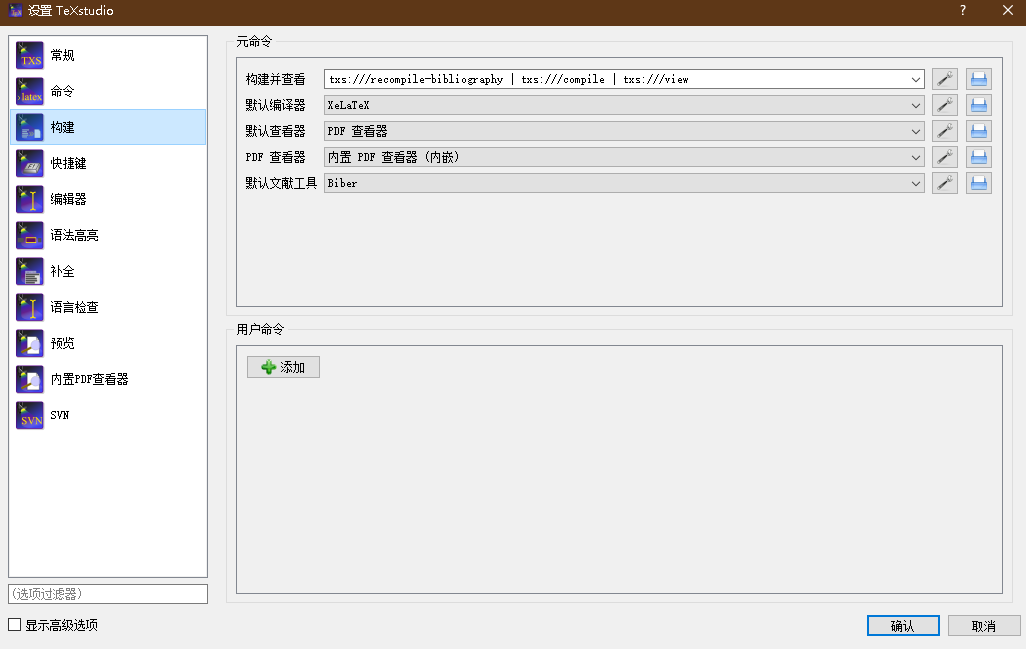
\includegraphics[scale=0.55]{Fig/TeXstudio.png}
	\caption{\label{TeXstudio}TeXstudio环境}
\end{figure}

\section{主文件}
scutthesis.tex文件相当于主函数,调用各章的内容。\LaTeX{}源代码以一个\textbackslash{}documentclass 命令作为开头,它指定了文档使用的文档类。文档类规定了\LaTeX{}源代码所要生成的文档的性质——普通文章、书籍、演示文稿、个人简
历等等。
\begin{lstlisting}
\documentclass[⟨options⟩]{⟨class-name⟩}
\end{lstlisting}
其中class-name为文档类的名称,如\LaTeX{}提供的article, book, report,可在其基础上派
生的一些文档类或者有其它功能的一些文档类。\LaTeX{}提供的基础文档类见文献\parencite{_c}。还可以自定义文档类,如华南理工大学硕博士论文文档类scutthesis,其实现保存在后缀名为.cls的文件中。可选参数options 为文档类指定选项。


document环境当中的内容是文档正文:
\begin{lstlisting}
\begin{document}
正文内容
\end{document}
\end{lstlisting}
正文中包含各章节内容:
\begin{lstlisting}
\chapter{摘\texorpdfstring{\quad}{}要}
	本模板由Shun Xu\cite{_}、yecfly\cite{_a}\added{以及mengchaoheng\cite{_mengChaoHeng}}的模板修改而来,适合于华南理工大学硕/博士毕业论文。
	既然已经入坑LaTeX,就不推荐使用LYX,但本模板在修改祖传代码过程中仅对修改部分进行更新,其余部分仍保留源代码。另外参考文献管理软件推荐使用zotero,这也是本模板使用的软件。
	本模板最主要的改动是参考文献使用biber,而不是原来的bibtex,因此不再需要.bst文件。
	\added{本模版更新了双盲评审选项,符合2022年最新的格式要求,将公式字体变更为Times New Roman等,具体细节见正文。}

\keywordsCN{\LaTeX{};论文}

\chapter{Abstract}
	

\keywordsEN{\LaTeX{}; Paper} % 中英文摘要
\tableofcontents	% 目录
\listoftables	% 表格目录(可选)
\listoffigures	% 插图目录(可选)
\include{symbols}	% 符号对照表(可选)
\include{abbreviation} 	% 缩略词	
...
\chapter{绪论}
%
\section{研究背景和意义}
\subsection{研究背景和意义}
%
关于\LaTeX{}以及基于\LaTeX{}写作的好处不再赘述。\LaTeX{}的入门资料推荐文献\parencite{_b}以及文献\parencite{_c}。

这里主要是想推荐一种“学术生态”,即利用各种工具展开科研工作,以达到事半功倍的效果。需要用到以下软件:
\begin{enumerate}
	\item 	参考文献管理软件zotero\cite{_f}。很多人使用过endnote,但其实zotero也非常强大,强烈推荐。可到b站观看Struggle with Me出品的视频教程\cite{_e}入门。\replaced{最新的zotero已支持软件内部PDF阅读。}{zotero不自带pdf阅读器,使用Adobe Acrobat pro DC即可。
				在Adobe中点击文件->属性->位置,即可打开文件所在位置,故亦不推荐更改zotero的文件系统。}
	\item	可截图获取文献中公式的软件mathpix\cite{_d}。在阅读别人的论文时,很可能需要把文章中的公式抄下来放到自己的笔记中,方便以后组会报告甚至论文中使用,这时使用mathpix可直接截图获取\LaTeX{}源码,非常方便。该软件普通邮箱注册可每月50次免费,学校邮箱可100次,若信用卡注册可1000次。	
	\item	\replaced{VS Code}{TeXstudio},相当于IDE。本模板是基于\replaced{VS Code}{TeXstudio2020}进行的,关于该软件的使用(快捷键等)可另行查找资料。\deleted{编译时可以使用该软件,也可以运行文件目录的all.bat。TeXstudio的设置见第二章。}
\end{enumerate}

\added{本文总体结构以及前三章均继承了前辈们的框架与内容,本人所做修改均标注为蓝色,第四章为本人撰写,故未作颜色标记。}本文的章节安排如下:

第一章,绪论。

第二章,模板简介。主要介绍各文件的内容。

第三章,常用环境。介绍论文写作中常用的环境,包括:图、表、公式、定理。基本涵盖了常用的命令。

\added{第四章,本人对前辈们的模版的修改之处,包括:双盲评审、图、公式、参考文献、标题等。}



	% 第一章
\chapter{模板简介}
%
与很多外文杂志社不同,大部分中文期刊都不提供\LaTeX{}模板给投稿者使用,也很少有学校给学生提供官方的毕业论文模板。目前github上的大部分模板都是由学生发起的非官方模板。在此感谢Shun Xu以及yecfly\added{、mengchaoheng}等人的工作,他们的无私贡献使得华南理工大学硕博士毕业论文也可以使用\LaTeX{}撰写。

本模板是直接修改前人的模板得到的,更详细的介绍可到\parencite{_,_a}下载。本章仅从用户的角度简要介绍模板的使用,而尽量避免涉及\LaTeX{}的模板制作细节(实际上是因为本人也不会)。正如我们使用手机并不需要了解麦克斯韦方程组,使用\LaTeX{}写作也无需了解模板是如何制作的。

\LaTeX{}的源代码保存在后缀名为.tex的文件中。当编写长篇文档时,例如当编写书籍、毕业论文时,单个源文件会使修改、校对变得十分困
难。将源文件分割成若干个文件,例如将每章内容单独写在一个文件中,会大大简化修改和校对
的工作。为方便,本文将scutthesis.tex文件称为主文件,而将abstract.tex、chapter0x.tex、conclusion.tex等文件称为章节文件。

值得注意的时,要每次编译时都更新参考文献著录,TeXstudio软件的选项->设置中的构建并查看、编译器需要设置成如图\ref{TeXstudio}所示。此时只需在任意一个文件中点击构建并查看按钮即可编译文档。每次编译都更新参考文献会使得编译时间很长。
\begin{figure}[htbp]
	\centering
	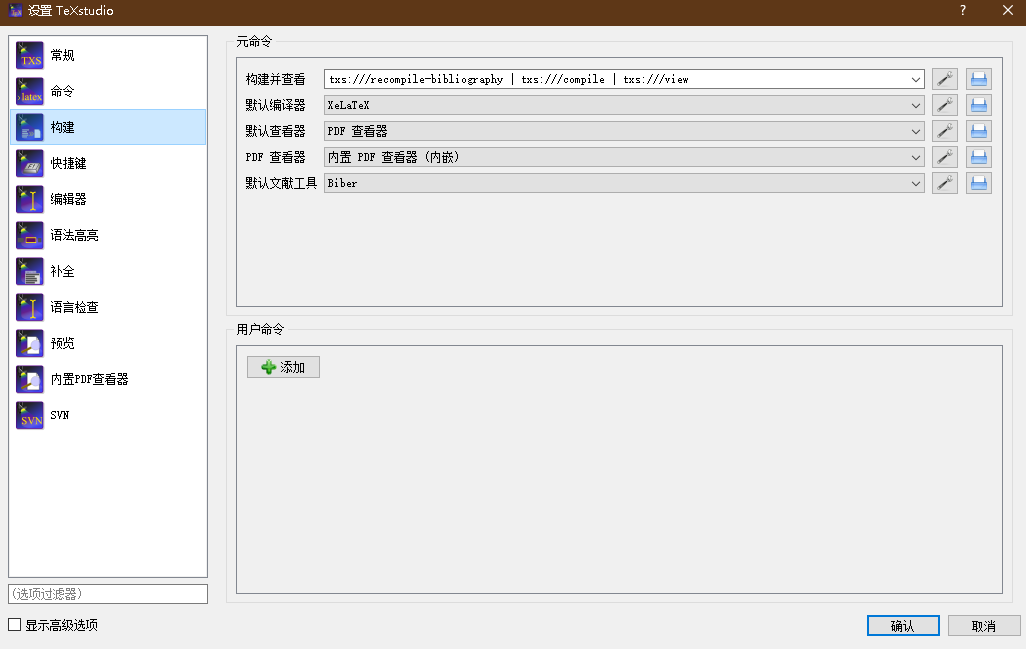
\includegraphics[scale=0.55]{Fig/TeXstudio.png}
	\caption{\label{TeXstudio}TeXstudio环境}
\end{figure}

\section{主文件}
scutthesis.tex文件相当于主函数,调用各章的内容。\LaTeX{}源代码以一个\textbackslash{}documentclass 命令作为开头,它指定了文档使用的文档类。文档类规定了\LaTeX{}源代码所要生成的文档的性质——普通文章、书籍、演示文稿、个人简
历等等。
\begin{lstlisting}
\documentclass[⟨options⟩]{⟨class-name⟩}
\end{lstlisting}
其中class-name为文档类的名称,如\LaTeX{}提供的article, book, report,可在其基础上派
生的一些文档类或者有其它功能的一些文档类。\LaTeX{}提供的基础文档类见文献\parencite{_c}。还可以自定义文档类,如华南理工大学硕博士论文文档类scutthesis,其实现保存在后缀名为.cls的文件中。可选参数options 为文档类指定选项。


document环境当中的内容是文档正文:
\begin{lstlisting}
\begin{document}
正文内容
\end{document}
\end{lstlisting}
正文中包含各章节内容:
\begin{lstlisting}
\include{abstract} % 中英文摘要
\tableofcontents	% 目录
\listoftables	% 表格目录(可选)
\listoffigures	% 插图目录(可选)
\include{symbols}	% 符号对照表(可选)
\include{abbreviation} 	% 缩略词	
...
\include{chapter01}	% 第一章
\include{chapter02} % 第二章
\include{chapter03} % 第三章
% 自行根据需要添加章节。
...
\include{conclusion} % 结论
...
\printbibliography	% 参考文献著录
\include{appendix} % 附录
\include{pub} % 成果
\include{ack} % 致谢
\end{lstlisting}
其中$\%$之后的内容为注释,...表示省略其他代码,仅保留论文内容主体部分。\textbackslash{}include\{xxx\}指令用于包含xxx.tex文件的内容,各章节的内容主要在xxx.tex中保存。在\textbackslash{}documentclass 和\textbackslash{}begin\{document\} 之间的位置称为导言区。在导言区中一般会使用\textbackslash{}usepackage 调用宏包,以及会进行对文档的全局设置。本模板的导言区除调用所需的宏包外,还进行了页眉页脚的设置。有的模板会把所有调用宏包的指令放到一个.sty宏包文件中,页面的设置放在文档类文件.cls文件中。因本人时间有限,就不做整理,欢迎有志之士加入完善。使用本模板并不需要了解导言区的指令,在需要时额外添加即可(要注意宏包冲突)。特别地,\textbackslash{}includeonly\{xxx\}指令用于使文档仅编译xxx.tex文件的内容,这就是分章节包含(include)的好处,可大大减少编译时间。

\replaced{封面内容可根据双盲评审论文模版.doc与doctor\_cover.doc另存为review\_cover.pdf或doctor\_cover.pdf,本模版会自动将其并入编译后的PDF文件。}{将封面打印保存为 doctor\_cover.pdf 文件,硕士使用master\_cover.docx ,博士使用 doctor\_cover.doc 。}如果有更新版本的封面,可自行替换。文档类默认是博士论文,下面指令将控制添加封面与否:
\begin{lstlisting}
\documentclass[unicode,master,pdfcover]{scutthesis}	% 使用pdf文件封面的 硕士模板
\documentclass[unicode,master]{scutthesis}	% 不使用pdf文件封面的 硕士模板
\documentclass[unicode,pdfcover]{scutthesis}	% 使用pdf文件封面的最终版博士学位论文模板
\documentclass[unicode]{scutthesis}	% 不使用pdf文件封面的博士模板
\documentclass[unicode,pdfcover,review]{scutthesis}	% 使用pdf文件封面的送审版的博士学位论文模版  revised by CYX
\end{lstlisting}
不使用doctor\_cover.pdf 文件指定的封面时,将使用草稿封面。草稿封面也可以减少编译时间,因此可以在最终提交论文时再使用论文封面。草稿封面用以下指令设置:
\begin{lstlisting}
%%%%%%%%%%%%%草稿封面设置%%%%%%%%%%%%%	
\title{LaTeX模板}	
\author{蒙超恒}	
\supervisor{指导教师:裴海龙\ 教授}	
\institute{华南理工大学}	
\date{2020年5月20日}
%%%%%%%%%%%%%%%%%%%%%%%%%%%%%%%%%%%%%
\end{lstlisting}
\section{章节文件}
章节文件如chapter0x.tex等,其内容由\textbackslash{}chapter\{章名\}开头。新建一章可新建一个文件并由\textbackslash{}chapter\{新建章名\}开头填写内容即可。节及小节分别用\textbackslash{}section\{新建节名\}、\textbackslash{}subsection\{新建小节名\}命令。

正文的的书写和txt文本文件的书写类似。\LaTeX{} 源代码中,空格键和Tab键输入的空白字符视为“空格”。连续的若干个空白字符视为一个空格。一行开头的空格忽略不计。行末的回车视为一个空格;但连续两个回车,也就是空行,会将文字分段。多个空行被视为一个空行。也可以在行末使用\textbackslash{}par 命令分段。在本模板中,英文之间的空格被保留,中文之间的空格被忽略。特别地,摘要,附录,结论等两个字的大纲级别为章的章名,中间使用空格隔开。对此论文撰写规范并没有明文要求,只是为了美观。也可以全部不加空格。一般情况下,在文本文字中添加空格使用\textbackslash{}quad命令,但由于文献\parencite{_i}所述原因,直接使用\textbackslash{}quad命令会报警,因而使用\textbackslash{}texorpdfstring\{\textbackslash{}quad\}\{\},其中最后一个\{\}里面可以加一个空格,不影响使用。目录二字之间添加空格在scutthesis.cls文件317行设置。

正文本环境中使用公式,即行内公式,需要用两个\$包围,如源码:\$a+b=c\$ 显示为$a+b=c$。使用其他字符可自行百度或阅读参考文献。再次提醒,使用\LaTeX{}撰写论文不需要研究其原理,在达到某种效果(图文显示、公式显示效果)时百度或查书寻找其代码即可。

综上,论文撰写只需要将自己的文本(包含行内公式)放到相应的章节处,并添加行间公式、图表环境并填写图表即可。行间公式、图表将在下一章介绍。

 % 第二章

\chapter{常用环境及参考文献设置}
强烈建议在使用公式、表格、定理环境时进行百度,没必要研究各种用法,只需要知道自己需要什么。因本人的论文所用表格较少,因而对表格不是很熟悉,本章对表格的介绍相应的较少。本章仅介绍本人在论文撰写过程中常用的环境以及参考文献设置。

\section{图}
图的导入需要提前准备好图片文件,最好是.png、.eps、.pdf或.jpg文件。另外,如果是从matlab导出图片文件,可使用print函数或手动导出,print函数的使用可参考“论文matlab作图程序"里的PlotToFileColorPDF.m文件。手动导出主要用于观察效果,可设置某种导出样式后导出该样式,下次使用时加载,具体可百度“matlab导出高清图片”。需要特别注意的是一定要1:1导入matlab生成的图片,并且图中文字设置好字体字号。

使用如下代码放置独立成行的图片,效果如图\ref{one_DFUAV}所示
\begin{lstlisting}
\begin{figure}[htbp]
	% 图片居中(列居中对齐)
	\centering	
	% 包含当前路径下的Fig文件夹的图片文件DFUAV_f31.png
	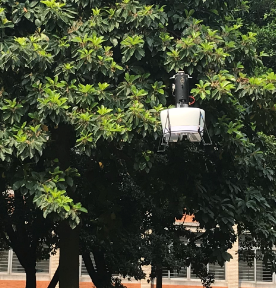
\includegraphics[scale=1]{Fig/DFUAV_f31.png} 
	% 添加标签one_DFUAV以及图标题“涵道风扇式无人机”,标题编号是自动生成的
	\caption{\label{one_DFUAV}涵道风扇式无人机} 
\end{figure}
\end{lstlisting}
其中figure为环境名,[htbp]表示将图片设置为浮动体,实际上这在.cls文件已经设置过,因而可以省略。[scale=1]表示安装1:1的比例导入图片,还可以按其他方式导入,需要时可自行百度。
\begin{figure}[htbp]
	\centering
	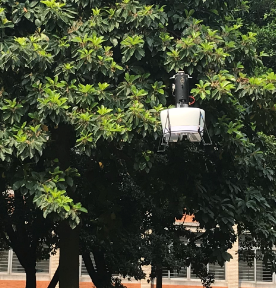
\includegraphics[scale=1]{Fig/DFUAV_f31.png}
	\caption{\label{one_DFUAV}涵道风扇式无人机}
\end{figure}

使用如下代码划分页面并排放置图\ref{Hawk}、图\ref{GTSpy}
\begin{lstlisting}
\begin{figure}[htbp]
	\centering
	\begin{minipage}[c]{0.5\textwidth} % minipage将页面划分为0.5\textwidth
		\centering
		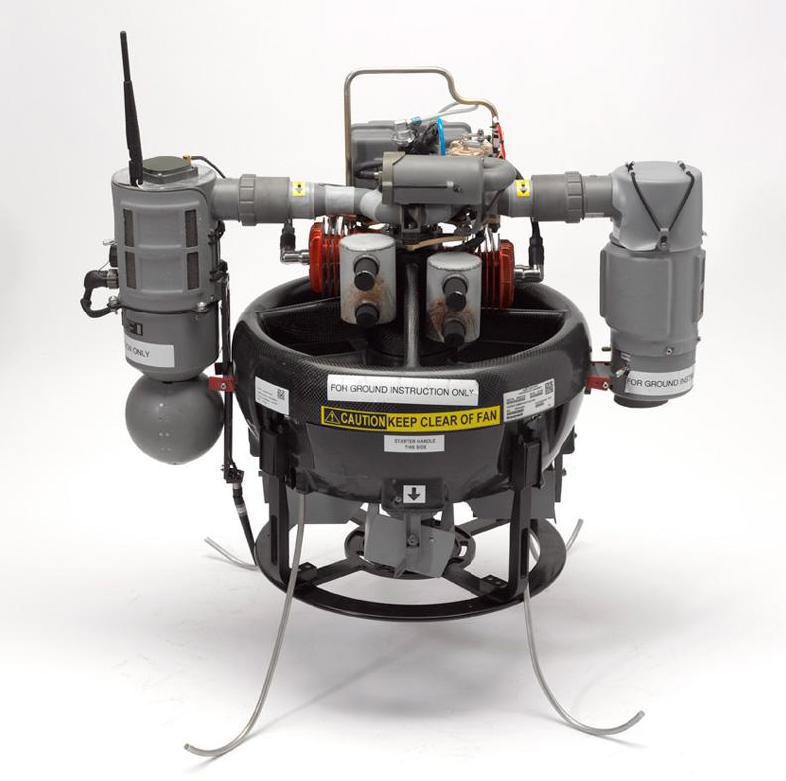
\includegraphics[width=6cm,height=6cm]{Fig/honeywell_t-hawk.jpg}
		\caption{\label{Hawk}T-Hawk}
	\end{minipage}%
	\begin{minipage}[c]{0.5\textwidth}
		\centering
		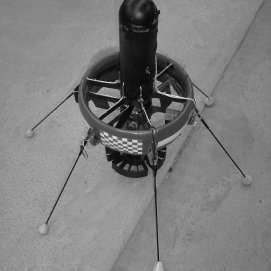
\includegraphics[width=6cm,height=6cm]{Fig/GTSpy.jpg}
		\caption{\label{GTSpy}GTSpy}
	\end{minipage}
\end{figure}
\end{lstlisting}
其中[c]表示行居中对齐。当图片大小不一但又需要1:1导入时,图标题可能行不对齐,因此可以改为如下指令:
\begin{lstlisting}
\begin{figure}[htbp]
	\centering
	\begin{minipage}[c]{0.5\textwidth}
		\centering
		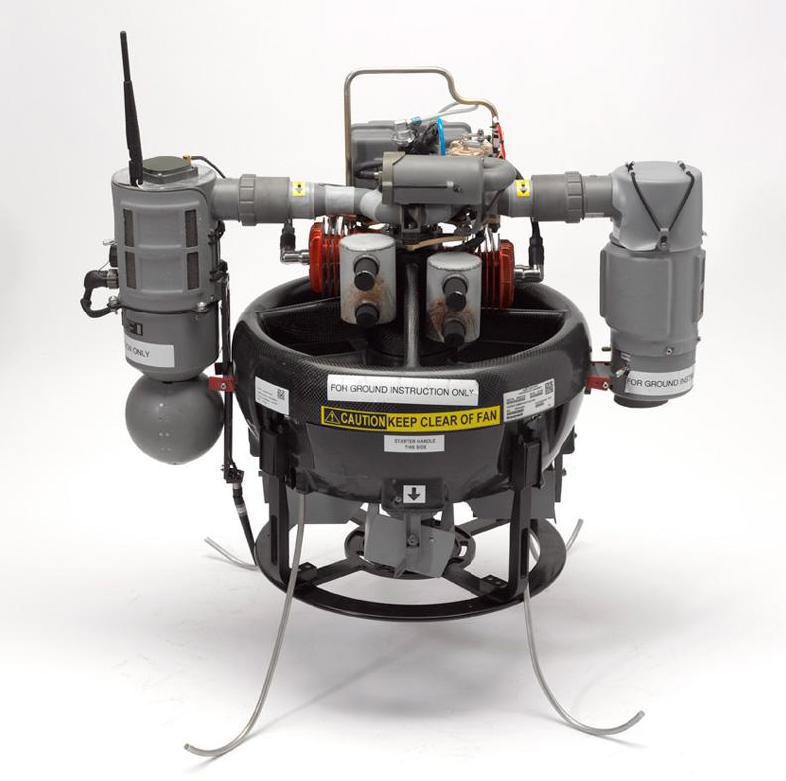
\includegraphics[scale=1]{Fig/honeywell_t-hawk.jpg} %1:1导入
	\end{minipage}%
	\begin{minipage}[c]{0.5\textwidth}
		\centering
		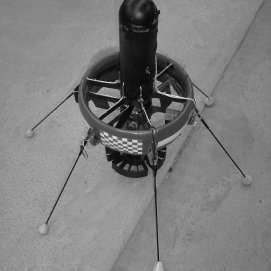
\includegraphics[scale=1]{Fig/GTSpy.jpg}
	\end{minipage}\\[1pt]
	\begin{minipage}[t]{0.5\textwidth}	% 以下为新添加页面划分,[t]表示行顶部对齐
		\caption{\label{Hawk}T-Hawk}
	\end{minipage}%
	\begin{minipage}[t]{0.5\textwidth}
		\caption{\label{GTSpy}GTSpy}
	\end{minipage}%
\end{figure}
\end{lstlisting}
\begin{figure}[htbp]
	\centering
	\begin{minipage}[c]{0.5\textwidth}
		\centering
		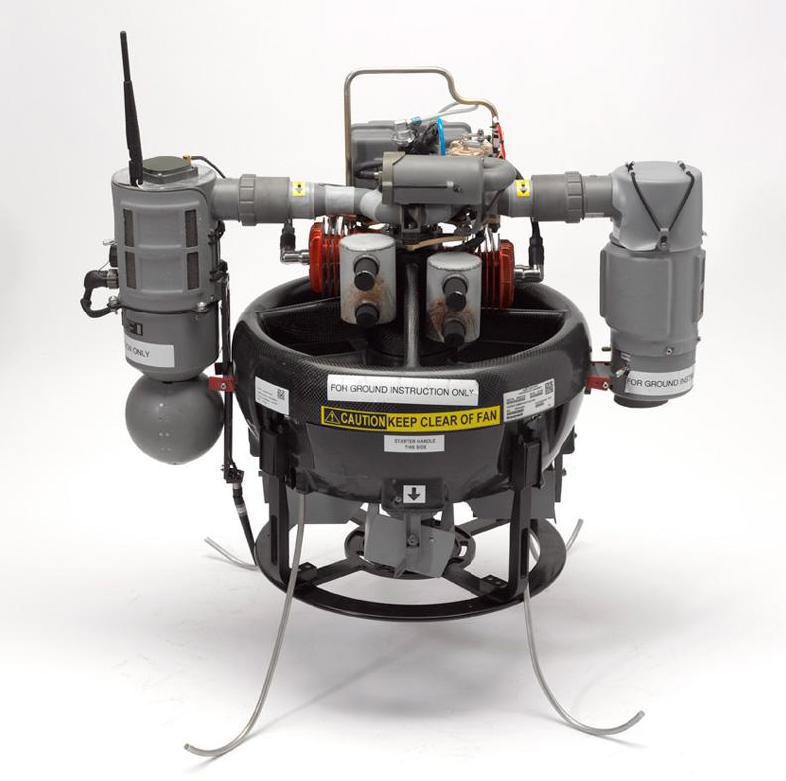
\includegraphics[width=6cm,height=6cm]{Fig/honeywell_t-hawk.jpg}
		\caption{\label{Hawk}T-Hawk}
	\end{minipage}%
	\begin{minipage}[c]{0.5\textwidth}
		\centering
		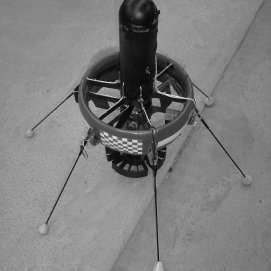
\includegraphics[width=6cm,height=6cm]{Fig/GTSpy.jpg}
		\caption{\label{GTSpy}GTSpy}
	\end{minipage}
\end{figure}
\section{表}
本节仅展示使用常见的三线表
\begin{lstlisting}
\begin{table}
	\caption{\label{TDF_para}涵道模型参数}	%表题在上
	\centering	% 表居中
	\small	% 表内字体小一号(即设置成和表题字号一致)
	\begin{tabular}{cccc}	% cccc表示4列并居中,若列之间需要分隔符则设置为|c|c|c|c|
		\hline	% \hline表示横线。列之间的元素用&分隔,\tabularnewline表示换行
		参数符号 & 数值 & 参数符号 & 数值 \tabularnewline 
		\hline 
		$I_x$ & $054593$ 		   & $I_y$ & $0.017045         $ \tabularnewline
		$l_1$ & $0.0808\,\text{m}$ & $l_2$ & $0.175\,\text{m}  $ \tabularnewline 
		$l_4$ & $0.2415\,\text{m}$ & $l_5$ & $0.1085\,\text{m} $ \tabularnewline
		\hline 
	\end{tabular}
\end{table}
\end{lstlisting}
\begin{table}
	\caption{\label{TDF_para}涵道模型参数}
	\centering
	\small 
	\begin{tabular}{cccc}
		\hline 
		参数符号 & 数值                & 参数符号 & 数值                 \tabularnewline
		\hline 
		$I_x$   & $054593$ 		     & $I_y$   & $0.017045         $ \tabularnewline
		$l_1$   & $0.0808\,\text{m}$ & $l_2$   & $0.175\,\text{m}  $ \tabularnewline 
		$l_4$   & $0.2415\,\text{m}$ & $l_5$   & $0.1085\,\text{m} $ \tabularnewline
		\hline 
	\end{tabular}
\end{table}
\added{表格的中英文题注,可以使用TableBicaption命令,与图片的用法一致}。
\section{公式}
除了前面讲行内公式,常用的还有行间公式。公式中的数学符号可自行百度,本章仅介绍常用的几种公式环境。

单独成行的行间公式在 \LaTeX{} 里由equation 环境包裹。equation 环境为公式自动生成一个编号,这个编号可以用\textbackslash{}label 和\textbackslash{}ref 生成交叉引用,amsmath 宏包的\textbackslash{}eqref 可为引用自动加上圆括号;如式\eqref{eq_1}所示。
\begin{lstlisting}
\begin{equation}
	a+b=c	\label{eq_1}
\end{equation}
\end{lstlisting}
\begin{equation}
	a+b=c	\label{eq_1}
\end{equation}
若不需要编号则加星号,改为
\begin{lstlisting}
\begin{equation*}
	a+b=c
\end{equation*}
\end{lstlisting}
其他环境类似。当使用 \texttt\$ 开启行内公式输入,或是使用{equation} 环境时,\LaTeX\ 就进入了数学模式。
数学模式相比于文本模式有以下特点:
\begin{enumerate}
	\item 数学模式中输入的空格被忽略。数学符号的间距默认由符号的性质(关系符号、运算符等)决定。
	需要人为引入间距时,使用 \textbackslash{}{quad} 和 \textbackslash{}{qquad} 等命令。
	\item {不允许有空行(分段)}。行间公式中也无法用 $ \verb|\\|$命令手动换行。排版多行公式需要用到 其他各种环境。
	\item 所有的字母被当作数学公式中的变量处理,字母间距与文本模式不一致,也无法生成单词之间的空格。
	如果想在数学公式中输入正体的文本,简单情况下可用 \textbackslash{}{mathrm} 命令。
	或者用 {amsmath} 提供的 \textbackslash{}{text} 命令(仅适合在公式中穿插少量文字。如果你的情况正好相反,需要在许多文字中穿插使用公式,则应该像正常的行内公式那样用,而不是滥用 \textbackslash{}{text} 命令)。
\end{enumerate}	

实际上更常用的的是多行公式,不需要对齐的公式组可以使用gather环境,需要对齐的公式组用align 环境。
长公式内可用$ \verb|\\|$ 换行。

如果需要罗列一系列公式,并令其按照等号对齐,可用align 环境,它将公式用\& 隔为两部分并对齐。分隔符通常放在等号左边:
\begin{lstlisting}
\begin{align}
	a & = b + c \\
	& = d + e
\end{align}
\end{lstlisting}
\begin{align}
a & = b + c \\
& = d + e
\end{align}
align 环境会给每行公式都编号。

如果不需要按等号对齐,只需罗列数个公式,可用gather环境:
\begin{lstlisting}
\begin{gather}
	a  = b + c \notag \\
	f = d + e 
\end{gather}
\end{lstlisting}
\begin{gather}
	a  = b + c \notag  \\
	f = d + e 
\end{gather}
gather 环境同样会给每行公式都编号,如果某行不需要编号可在行末用\textbackslash{}notag 仅去掉某行的编号。

align 和gather 有对应的不带编号的版本align* 和gather*。

另一个常见的需求是将多个公式组在一起公用一个编号,编号位于公式的居中位置。为此,
amsmath 宏包提供了诸如aligned、gathered 等环境,与equation 环境套用。以-ed 结尾的
环境用法与前一节不以-ed 结尾的环境用法一一对应。我们仅以aligned 举例:
\begin{lstlisting}
\begin{equation}
	\begin{aligned}
		a &= b + c \\
		d &= e + f + g \\
		h + i &= j + k \\
		l + m &= n
	\end{aligned}
\end{equation}
\end{lstlisting}
\begin{equation}
	\begin{aligned}
		a &= b + c \\
		d &= e + f + g \\
		h + i &= j + k \\
		l + m &= n
	\end{aligned}
\end{equation}
split 环境和aligned 环境用法类似,也用于和equation 环境套用,区别是split 只能
将每行的一个公式分两栏,aligned 允许每行多个公式多栏。

分段函数通常用amsmath 宏包提供的cases 环境,可参考文献\parencite{_c}

amsmath 宏包还直接提供了多种排版矩阵的环境,包括不带定界符的matrix,以及带各种定界符的矩阵pmatrix、bmatrix、Bmatrix、vmatrix、Vmatrix。
其中中括号版的bmatrix最常用。这些矩阵环境需要在公式中使用,比如 align 环境。
\begin{lstlisting}
A= \begin{bmatrix}
		x_{11} & x_{12} & \ldots & x_{1n} \\
		x_{21} & x_{22} & \ldots & x_{2n} \\
		\vdots & \vdots & \ddots & \vdots \\
		x_{n1} & x_{n2} & \ldots & x_{nn}
	\end{bmatrix}
\end{gather}
\end{lstlisting}
\begin{gather}
\bm{A}= \begin{bmatrix}
	x_{11} & x_{12} & \ldots & x_{1n} \\
	x_{21} & x_{22} & \ldots & x_{2n} \\
	\vdots & \vdots & \ddots & \vdots \\
	x_{n1} & x_{n2} & \ldots & x_{nn}
   \end{bmatrix}
\end{gather}	
其中矩阵/向量加粗使用\textbackslash{}bm\{\}命令。另外还可以使用array环境排版矩阵,类似tabular环境,用$ \verb|\\|$ 和\& 用来分隔行和列,这里不再赘述。	
\begin{lstlisting}
\begin{array }[外部对齐tcb]{列对齐lcr}
	行列内容
\end{array}
\end{lstlisting}

另外注意排版分式时,有两种方法:\textbackslash{}frac或者\textbackslash{}dfrac,效果分别为$ \frac{1}{2} $和$ \dfrac{1}{2} $。以上介绍的数学环境中,空格可参考文献\parencite{_c},例如常用\textbackslash{}quad。
\section{定理}
在scutthesis.cls文件536行开始,已经用\textbackslash{}newtheorem命令定义了几种定理环境,包括:定义、假设、定理、结论、引理、公理、推论、性质等等,统称定理环境,关于\textbackslash{}newtheorem的用法,可参考\cite{_c}或自行百度。要下面提供几个例子,在横线之间的深色区域是代码,效果在相应下方表示:
\begin{lstlisting}
\begin{assumption}
	加权矩阵${{\bm{W}}_{1}}$和 ${{\bm{W}}_{2}}$ 是对称矩阵,且$ {{\bm{W}}_{2}}$非奇异。	\label{assum_dca1}
\end{assumption}
\end{lstlisting}
\begin{assumption}
	加权矩阵${{\bm{W}}_{1}}$和 ${{\bm{W}}_{2}}$ 是对称矩阵,且$ {{\bm{W}}_{2}}$非奇异。	\label{assum_dca1}
\end{assumption}

定理用法和假设类似:
\begin{lstlisting}
\begin{theorem}
	如果假设\ref{assum_dca1}成立,$\bm{F}$满足式\eqref{eq_F}的定义,且${{\bm{W}}_{1}}$非奇异,则有$0\le e \left( \bm{F} \right) < 1$,其中$e \left( \bm{F} \right)$是 $\bm{F}$的特征值。	\label{the_dca2}
\end{theorem}
\end{lstlisting}
\begin{theorem}
	如果假设\ref{assum_dca1}成立,$\bm{F}$满足上式的定义,且${{\bm{W}}_{1}}$非奇异,则有$0\le e \left( \bm{F} \right) < 1$,其中$e \left( \bm{F} \right)$是 $\bm{F}$的特征值。	\label{the_dca2}
\end{theorem}

定理环境的编号可自定义,但通常不需要再进行设置,因为模板文件scutthesis.cls文件已经定义好。
\section{参考文献}

\begin{lstlisting}
关于参考文献这块,很多同学有疑问。只有记住一点:不管用什么参考文献管理工具,最终目的是生成一个bib文件给TeXstudio使用,bib文件里是特定格式的文献信息。bib文件可以使用一个叫notepad++的软件打开。
\end{lstlisting}

通常学位论文参考文献是基于BibTeX进行的,本模板最大的改进就是引入BibLaTeX。关于这部分知识可参考文献\cite{_c}的第六章,6.1节参考文献和BIBTEX工具。

参考文献引用和著录是基于ZOTERO这个软件进行的。视频教程见\parencite{_e}。此外,为了符合毕业论文撰写规范,需设置参数。按照视频教程安装完必要的插件(如Better BibTeX)后,在编辑->首选项进行设置。附录图\ref{op1}到图\ref{op11}所示的是我的zotero软件设置。其中最重要的是\ref{op10}的设置要排除的选项,多余的显示会让审稿人反感,按照论文撰写规范进行即可。在毕业论文撰写时,在编辑->首选项->Better BibLTeX->Fields中,Fields to omit from export填month,abstract,note,extra,file,keywords,type,url,doi,就是在参考文献著录中排除这些多余的项,避免过于复杂。而在写本模板使用说明时,没有排除url,因为很多参考资料是网页。

\begin{lstlisting}
使用zotero,科学上网很重要,通常我们使用谷歌学术搜索文献并利用chrome的zotero插件直接捕获文献著录信息。但我使用蓝灯,代理服务器均遇到过被谷歌学术封锁的情况。只能不断换科学上网方法。这里我现在用的chrome插件:谷歌上网助手,它可以轻松捕获谷歌学术的著录信息,注册一个账号即可使用。谷歌上网助手有可能和某些代理冲突。这些都是科学上网的问题,已经超出了本项目的范围,听说百度一下 v2ray 可发现新大陆,可惜我试了Vultr的服务器依然被谷歌封。知网捕获中文参考文献著录信息的话不需要考虑这个问题,直接在知网首页搜索文献然后点击插件既可以选想捕获的著录了。
\end{lstlisting}

在zotero软件点击文件->导出文献库,如图\ref{output}所示,再在导出对话框图\ref{output_format}选择导出格式为Better BibLaTeX,同时勾选Keep updated选项保持自动更新,再点击ok,在弹出的对话框图\ref{output_name}确定保存路径和文件名,例如我的是MyLibrary.bib,这也是我整个读书生涯的文献库bib文件。如果写小论文的话通常导出格式是BibTeX或者Better BibTeX(这里按照期刊的要求来即可,文献管理软件的好处就是快速自动生成一个文件库)。关于BibTeX和BibLaTeX的区别这里不做展开。

得到文献库后,在scutthesis.tex文件第九行使用\textbackslash{}addbibresource命令,添加文献库。引用某文献时秩序在zotero选中某文献条目,然后按Ctrl+Shift+C,复制引用关键字(Citation Key)到剪切板(快捷键可自定义)。然后在tex文件编辑界面直接粘贴,默认的时上标形式,若需要非上标形式,可以改为\textbackslash{}parencite{XXXX},其中XXXX是Citation Key。这里的操作和认为设置的首选项参数有关,需要在编辑->首选项->导出界面的默认格式一栏选中相应的项,同时在编辑->首选项->高级->快捷键设置为默认值。

---------------------------------------------------------------------------------

2020年12月2日测试:
下载最新zotero,从知网和谷歌捕获文献(刚打开网页最好稍等一会再点击插件,谷歌可能需要现人机验证),对文献\parencite{Renduchintala_2019}、\parencite{Meng_2020}进行引用。

---------------------------------------------------------------------------------
\begin{lstlisting}
另外有同学反映,换了电脑后重新导出的bib文件Citation Key值不同,记得设置好Better BibTeX之后,在著录条目界面全选著录(或仅选想更新的著录)然后右键选Better BibTeX更新refresh一下。然后在Automatic export选项点击Export now立即更新bib文件(按理说勾选了自动更新选项他会自动更新,但为了确保万无一失还是点一下)。
\end{lstlisting}










 % 第三章
% 自行根据需要添加章节。
...
\chapter{结\texorpdfstring{\quad}{}论}
本文主要是展示如何使用修改“祖传模板”得到的新模板,在使用时直接替换成自己的论文内容即可。总结下来最最最麻烦的是科学上网,只有科学上网才能获取文献信息生成bib文件,后面就好办了。

本模板难免有不足之处,主要是我本人的论文涉及的格式有限,有些地方没探索到自然就没去设置。比如附录,附录的图文并茂等等,我本人是没有研究的,这里仅仅做了一些初步的工作,不过对很多同学来说本模板是够用的。希望有能帮助到华工的同学们,有不足之处请多多理解,可以通过邮件联系我,上班之余我会尽量回复。 % 结论
...
\printbibliography	% 参考文献著录
\include{appendix} % 附录
\chapter{攻读博士学位期间取得的研究成果}

一、已发表(包括已接受待发表)的论文,以及已投稿、或已成文打算投稿、或拟成文投稿的论文情况\underline{\textbf{(只填写与学位论文内容相关的部分):}}

\begin{centering}
	\small
	\begin{longtable}{|>{\centering}m{0.5cm}|>{\centering}m{2.2cm}|>{\centering}m{3.3cm}|>{\centering}m{2.7cm}|>{\centering}m{1.8cm}|>{\centering}m{1.8cm}|>{\centering}m{1cm}|}
		\hline 
		\textbf{序号} & \textbf{作者} & \textbf{题\qquad 目} 						   & \textbf{发表或投稿刊物名称、级别} & \textbf{发表的卷期、年月、页码} & \textbf{与学位论文哪一部分(章、节)相关} & \textbf{被索引收录情况}\tabularnewline
		\hline 
		1   & \textbf{Cui Yanxin}, Kang Youping,\\ Shi Yonghua, Chen Jinrong, Wang Zishun, Wang Jinyi & Investigation into the arc profiles and penetration ability of axial magnetic field-enhanced K-TIG welding by means of a specially designed sandwich & Journal of Manufacturing Processes\\(IF:5.01, JCR Q2) & 2021, 68:32-41 & 第五章 & SCI\tabularnewline
		\hline 
		2	& \textbf{Cui Yanxin}, Shi Yonghua, Hong Xiaobin & To be continued & Journal of Manufacturing Processes\\(IF:5.01, JCR Q2)  & 2019, 46:225-233 & 第六章 &SCI \tabularnewline
		\hline
	\end{longtable}
\end{centering}
\newpage
二、与学位内容相关的其它成果(包括专利、著作、获奖项目等)

1、与学位内容相关的著作

\begin{centering}
	\small
	\begin{longtable}{|>{\centering}m{0.5cm}|>{\centering}m{2.2cm}|>{\centering}m{4.7cm}|>{\centering}m{2.7cm}|>{\centering}m{1.8cm}|>{\centering}m{1.8cm}|}
		\hline 
		\textbf{序号} & \textbf{作者} & \textbf{著作名称} 						   & \textbf{出版社} & \textbf{出版的年月、页码} & \textbf{与学位论文哪一部分(章、节)相关} \tabularnewline
		\hline 
		1	& Shi Yonghua, \textbf{Cui Yanxin}, Cui Shuwan, Zhang Baori & A Novel High-Efficiency Keyhole Tungsten Inert Gas (K-TIG) Welding: Principles and Practices & Welding Technology. Cham: Springer International Publishing & 2021: 313–367 & 第三章\\第六章\tabularnewline
		\hline
	\end{longtable}
\end{centering}

2、与学位内容相关的专利

\begin{centering}
	\small
	\begin{longtable}{|>{\centering}m{0.5cm}|>{\centering}m{4cm}|>{\centering}m{3.5cm}|>{\centering}m{4cm}|>{\centering}m{2.2cm}|}
		\hline
		\textbf{序号}	&	\textbf{专利申请人}	&	\textbf{专利名称}	&	\textbf{专利号}	&	\textbf{与学位论文哪一部分(章、节)相关}\tabularnewline
		\hline
		1	& 石永华,\textbf{崔延鑫},陈金荣,陈云可	&	一种用于锁孔效应深熔TIG焊的电弧压力测量装置与方法	&	发明专利202110489846.6(已授权)	& 第二章\tabularnewline
		\hline
		2	& ***	& 	***	& ***	& 第二章\tabularnewline
		\hline
	\end{longtable}
\end{centering} % 成果
\chapter{致\texorpdfstring{\quad}{}谢}
%把下面文字替换
感谢各位前辈提供的模版!

%把上面文字替换

~\\

\begin{minipage}[t]{0.945\textwidth}%
	\begin{flushright}
		崔延鑫\\
		\today\\	% 自动时间
		%2022年4月6日\\	%固定时间
		于华南理工大学
		\par\end{flushright}
\end{minipage}

 % 致谢
\end{lstlisting}
其中$\%$之后的内容为注释,...表示省略其他代码,仅保留论文内容主体部分。\textbackslash{}include\{xxx\}指令用于包含xxx.tex文件的内容,各章节的内容主要在xxx.tex中保存。在\textbackslash{}documentclass 和\textbackslash{}begin\{document\} 之间的位置称为导言区。在导言区中一般会使用\textbackslash{}usepackage 调用宏包,以及会进行对文档的全局设置。本模板的导言区除调用所需的宏包外,还进行了页眉页脚的设置。有的模板会把所有调用宏包的指令放到一个.sty宏包文件中,页面的设置放在文档类文件.cls文件中。因本人时间有限,就不做整理,欢迎有志之士加入完善。使用本模板并不需要了解导言区的指令,在需要时额外添加即可(要注意宏包冲突)。特别地,\textbackslash{}includeonly\{xxx\}指令用于使文档仅编译xxx.tex文件的内容,这就是分章节包含(include)的好处,可大大减少编译时间。

\replaced{封面内容可根据双盲评审论文模版.doc与doctor\_cover.doc另存为review\_cover.pdf或doctor\_cover.pdf,本模版会自动将其并入编译后的PDF文件。}{将封面打印保存为 doctor\_cover.pdf 文件,硕士使用master\_cover.docx ,博士使用 doctor\_cover.doc 。}如果有更新版本的封面,可自行替换。文档类默认是博士论文,下面指令将控制添加封面与否:
\begin{lstlisting}
\documentclass[unicode,master,pdfcover]{scutthesis}	% 使用pdf文件封面的 硕士模板
\documentclass[unicode,master]{scutthesis}	% 不使用pdf文件封面的 硕士模板
\documentclass[unicode,pdfcover]{scutthesis}	% 使用pdf文件封面的最终版博士学位论文模板
\documentclass[unicode]{scutthesis}	% 不使用pdf文件封面的博士模板
\documentclass[unicode,pdfcover,review]{scutthesis}	% 使用pdf文件封面的送审版的博士学位论文模版  revised by CYX
\end{lstlisting}
不使用doctor\_cover.pdf 文件指定的封面时,将使用草稿封面。草稿封面也可以减少编译时间,因此可以在最终提交论文时再使用论文封面。草稿封面用以下指令设置:
\begin{lstlisting}
%%%%%%%%%%%%%草稿封面设置%%%%%%%%%%%%%	
\title{LaTeX模板}	
\author{蒙超恒}	
\supervisor{指导教师:裴海龙\ 教授}	
\institute{华南理工大学}	
\date{2020年5月20日}
%%%%%%%%%%%%%%%%%%%%%%%%%%%%%%%%%%%%%
\end{lstlisting}
\section{章节文件}
章节文件如chapter0x.tex等,其内容由\textbackslash{}chapter\{章名\}开头。新建一章可新建一个文件并由\textbackslash{}chapter\{新建章名\}开头填写内容即可。节及小节分别用\textbackslash{}section\{新建节名\}、\textbackslash{}subsection\{新建小节名\}命令。

正文的的书写和txt文本文件的书写类似。\LaTeX{} 源代码中,空格键和Tab键输入的空白字符视为“空格”。连续的若干个空白字符视为一个空格。一行开头的空格忽略不计。行末的回车视为一个空格;但连续两个回车,也就是空行,会将文字分段。多个空行被视为一个空行。也可以在行末使用\textbackslash{}par 命令分段。在本模板中,英文之间的空格被保留,中文之间的空格被忽略。特别地,摘要,附录,结论等两个字的大纲级别为章的章名,中间使用空格隔开。对此论文撰写规范并没有明文要求,只是为了美观。也可以全部不加空格。一般情况下,在文本文字中添加空格使用\textbackslash{}quad命令,但由于文献\parencite{_i}所述原因,直接使用\textbackslash{}quad命令会报警,因而使用\textbackslash{}texorpdfstring\{\textbackslash{}quad\}\{\},其中最后一个\{\}里面可以加一个空格,不影响使用。目录二字之间添加空格在scutthesis.cls文件317行设置。

正文本环境中使用公式,即行内公式,需要用两个\$包围,如源码:\$a+b=c\$ 显示为$a+b=c$。使用其他字符可自行百度或阅读参考文献。再次提醒,使用\LaTeX{}撰写论文不需要研究其原理,在达到某种效果(图文显示、公式显示效果)时百度或查书寻找其代码即可。

综上,论文撰写只需要将自己的文本(包含行内公式)放到相应的章节处,并添加行间公式、图表环境并填写图表即可。行间公式、图表将在下一章介绍。

 % 第二章

\chapter{常用环境及参考文献设置}
强烈建议在使用公式、表格、定理环境时进行百度,没必要研究各种用法,只需要知道自己需要什么。因本人的论文所用表格较少,因而对表格不是很熟悉,本章对表格的介绍相应的较少。本章仅介绍本人在论文撰写过程中常用的环境以及参考文献设置。

\section{图}
图的导入需要提前准备好图片文件,最好是.png、.eps、.pdf或.jpg文件。另外,如果是从matlab导出图片文件,可使用print函数或手动导出,print函数的使用可参考“论文matlab作图程序"里的PlotToFileColorPDF.m文件。手动导出主要用于观察效果,可设置某种导出样式后导出该样式,下次使用时加载,具体可百度“matlab导出高清图片”。需要特别注意的是一定要1:1导入matlab生成的图片,并且图中文字设置好字体字号。

使用如下代码放置独立成行的图片,效果如图\ref{one_DFUAV}所示
\begin{lstlisting}
\begin{figure}[htbp]
	% 图片居中(列居中对齐)
	\centering	
	% 包含当前路径下的Fig文件夹的图片文件DFUAV_f31.png
	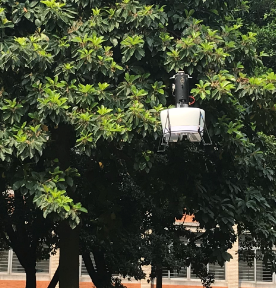
\includegraphics[scale=1]{Fig/DFUAV_f31.png} 
	% 添加标签one_DFUAV以及图标题“涵道风扇式无人机”,标题编号是自动生成的
	\caption{\label{one_DFUAV}涵道风扇式无人机} 
\end{figure}
\end{lstlisting}
其中figure为环境名,[htbp]表示将图片设置为浮动体,实际上这在.cls文件已经设置过,因而可以省略。[scale=1]表示安装1:1的比例导入图片,还可以按其他方式导入,需要时可自行百度。
\begin{figure}[htbp]
	\centering
	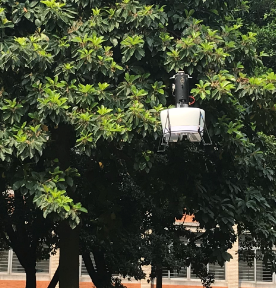
\includegraphics[scale=1]{Fig/DFUAV_f31.png}
	\caption{\label{one_DFUAV}涵道风扇式无人机}
\end{figure}

使用如下代码划分页面并排放置图\ref{Hawk}、图\ref{GTSpy}
\begin{lstlisting}
\begin{figure}[htbp]
	\centering
	\begin{minipage}[c]{0.5\textwidth} % minipage将页面划分为0.5\textwidth
		\centering
		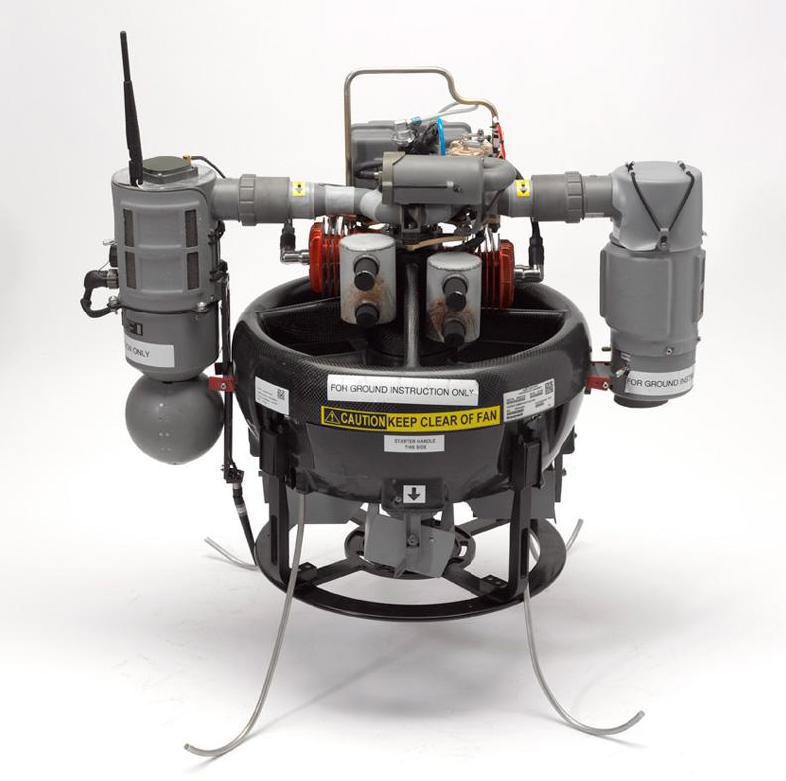
\includegraphics[width=6cm,height=6cm]{Fig/honeywell_t-hawk.jpg}
		\caption{\label{Hawk}T-Hawk}
	\end{minipage}%
	\begin{minipage}[c]{0.5\textwidth}
		\centering
		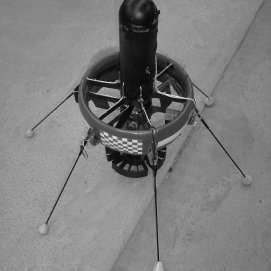
\includegraphics[width=6cm,height=6cm]{Fig/GTSpy.jpg}
		\caption{\label{GTSpy}GTSpy}
	\end{minipage}
\end{figure}
\end{lstlisting}
其中[c]表示行居中对齐。当图片大小不一但又需要1:1导入时,图标题可能行不对齐,因此可以改为如下指令:
\begin{lstlisting}
\begin{figure}[htbp]
	\centering
	\begin{minipage}[c]{0.5\textwidth}
		\centering
		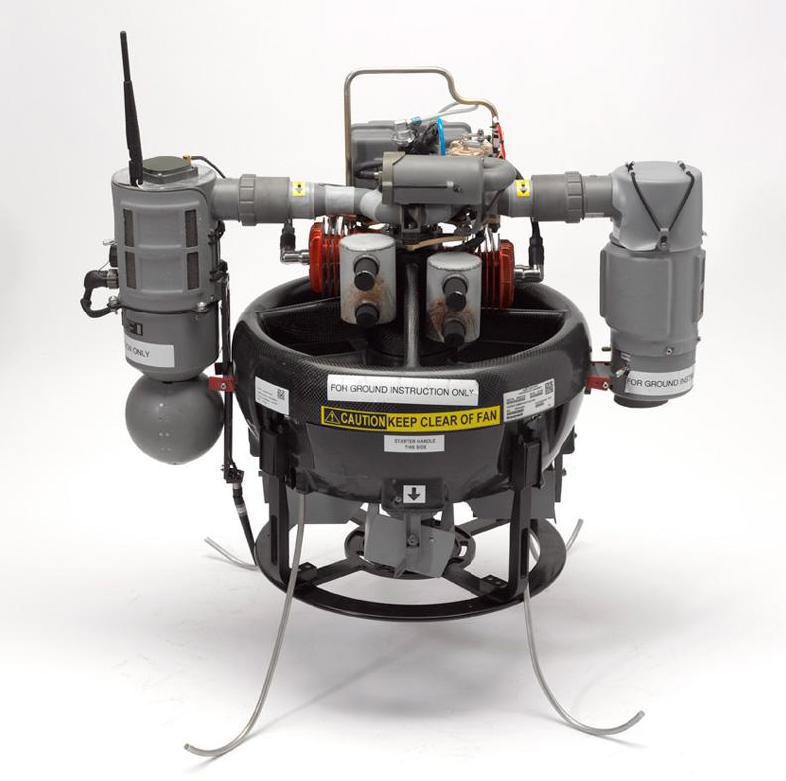
\includegraphics[scale=1]{Fig/honeywell_t-hawk.jpg} %1:1导入
	\end{minipage}%
	\begin{minipage}[c]{0.5\textwidth}
		\centering
		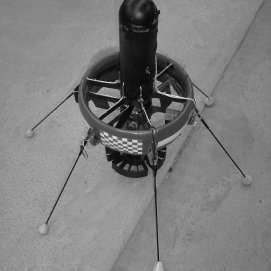
\includegraphics[scale=1]{Fig/GTSpy.jpg}
	\end{minipage}\\[1pt]
	\begin{minipage}[t]{0.5\textwidth}	% 以下为新添加页面划分,[t]表示行顶部对齐
		\caption{\label{Hawk}T-Hawk}
	\end{minipage}%
	\begin{minipage}[t]{0.5\textwidth}
		\caption{\label{GTSpy}GTSpy}
	\end{minipage}%
\end{figure}
\end{lstlisting}
\begin{figure}[htbp]
	\centering
	\begin{minipage}[c]{0.5\textwidth}
		\centering
		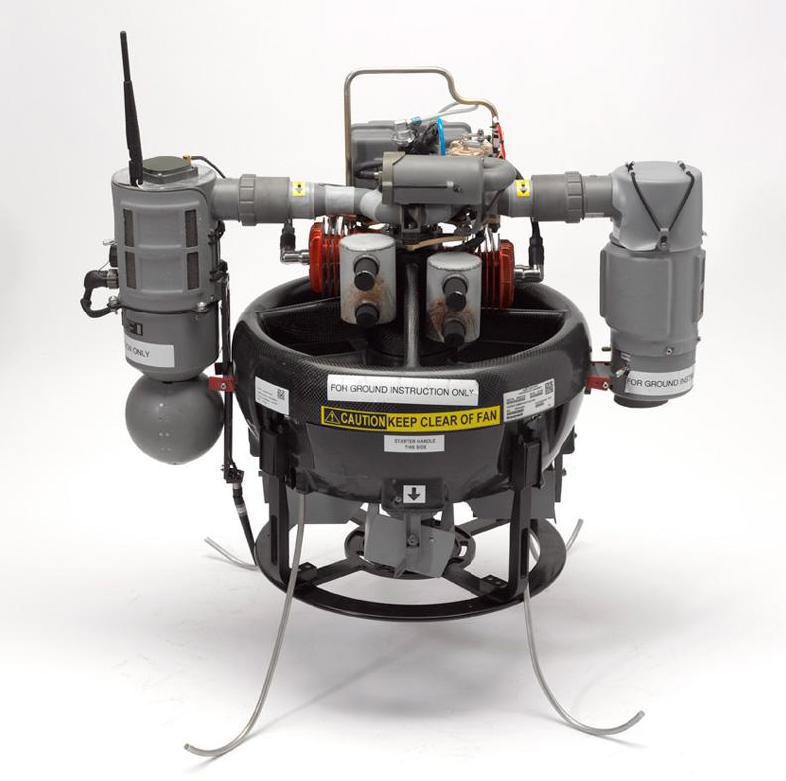
\includegraphics[width=6cm,height=6cm]{Fig/honeywell_t-hawk.jpg}
		\caption{\label{Hawk}T-Hawk}
	\end{minipage}%
	\begin{minipage}[c]{0.5\textwidth}
		\centering
		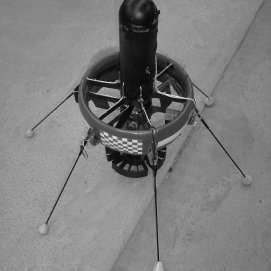
\includegraphics[width=6cm,height=6cm]{Fig/GTSpy.jpg}
		\caption{\label{GTSpy}GTSpy}
	\end{minipage}
\end{figure}
\section{表}
本节仅展示使用常见的三线表
\begin{lstlisting}
\begin{table}
	\caption{\label{TDF_para}涵道模型参数}	%表题在上
	\centering	% 表居中
	\small	% 表内字体小一号(即设置成和表题字号一致)
	\begin{tabular}{cccc}	% cccc表示4列并居中,若列之间需要分隔符则设置为|c|c|c|c|
		\hline	% \hline表示横线。列之间的元素用&分隔,\tabularnewline表示换行
		参数符号 & 数值 & 参数符号 & 数值 \tabularnewline 
		\hline 
		$I_x$ & $054593$ 		   & $I_y$ & $0.017045         $ \tabularnewline
		$l_1$ & $0.0808\,\text{m}$ & $l_2$ & $0.175\,\text{m}  $ \tabularnewline 
		$l_4$ & $0.2415\,\text{m}$ & $l_5$ & $0.1085\,\text{m} $ \tabularnewline
		\hline 
	\end{tabular}
\end{table}
\end{lstlisting}
\begin{table}
	\caption{\label{TDF_para}涵道模型参数}
	\centering
	\small 
	\begin{tabular}{cccc}
		\hline 
		参数符号 & 数值                & 参数符号 & 数值                 \tabularnewline
		\hline 
		$I_x$   & $054593$ 		     & $I_y$   & $0.017045         $ \tabularnewline
		$l_1$   & $0.0808\,\text{m}$ & $l_2$   & $0.175\,\text{m}  $ \tabularnewline 
		$l_4$   & $0.2415\,\text{m}$ & $l_5$   & $0.1085\,\text{m} $ \tabularnewline
		\hline 
	\end{tabular}
\end{table}
\added{表格的中英文题注,可以使用TableBicaption命令,与图片的用法一致}。
\section{公式}
除了前面讲行内公式,常用的还有行间公式。公式中的数学符号可自行百度,本章仅介绍常用的几种公式环境。

单独成行的行间公式在 \LaTeX{} 里由equation 环境包裹。equation 环境为公式自动生成一个编号,这个编号可以用\textbackslash{}label 和\textbackslash{}ref 生成交叉引用,amsmath 宏包的\textbackslash{}eqref 可为引用自动加上圆括号;如式\eqref{eq_1}所示。
\begin{lstlisting}
\begin{equation}
	a+b=c	\label{eq_1}
\end{equation}
\end{lstlisting}
\begin{equation}
	a+b=c	\label{eq_1}
\end{equation}
若不需要编号则加星号,改为
\begin{lstlisting}
\begin{equation*}
	a+b=c
\end{equation*}
\end{lstlisting}
其他环境类似。当使用 \texttt\$ 开启行内公式输入,或是使用{equation} 环境时,\LaTeX\ 就进入了数学模式。
数学模式相比于文本模式有以下特点:
\begin{enumerate}
	\item 数学模式中输入的空格被忽略。数学符号的间距默认由符号的性质(关系符号、运算符等)决定。
	需要人为引入间距时,使用 \textbackslash{}{quad} 和 \textbackslash{}{qquad} 等命令。
	\item {不允许有空行(分段)}。行间公式中也无法用 $ \verb|\\|$命令手动换行。排版多行公式需要用到 其他各种环境。
	\item 所有的字母被当作数学公式中的变量处理,字母间距与文本模式不一致,也无法生成单词之间的空格。
	如果想在数学公式中输入正体的文本,简单情况下可用 \textbackslash{}{mathrm} 命令。
	或者用 {amsmath} 提供的 \textbackslash{}{text} 命令(仅适合在公式中穿插少量文字。如果你的情况正好相反,需要在许多文字中穿插使用公式,则应该像正常的行内公式那样用,而不是滥用 \textbackslash{}{text} 命令)。
\end{enumerate}	

实际上更常用的的是多行公式,不需要对齐的公式组可以使用gather环境,需要对齐的公式组用align 环境。
长公式内可用$ \verb|\\|$ 换行。

如果需要罗列一系列公式,并令其按照等号对齐,可用align 环境,它将公式用\& 隔为两部分并对齐。分隔符通常放在等号左边:
\begin{lstlisting}
\begin{align}
	a & = b + c \\
	& = d + e
\end{align}
\end{lstlisting}
\begin{align}
a & = b + c \\
& = d + e
\end{align}
align 环境会给每行公式都编号。

如果不需要按等号对齐,只需罗列数个公式,可用gather环境:
\begin{lstlisting}
\begin{gather}
	a  = b + c \notag \\
	f = d + e 
\end{gather}
\end{lstlisting}
\begin{gather}
	a  = b + c \notag  \\
	f = d + e 
\end{gather}
gather 环境同样会给每行公式都编号,如果某行不需要编号可在行末用\textbackslash{}notag 仅去掉某行的编号。

align 和gather 有对应的不带编号的版本align* 和gather*。

另一个常见的需求是将多个公式组在一起公用一个编号,编号位于公式的居中位置。为此,
amsmath 宏包提供了诸如aligned、gathered 等环境,与equation 环境套用。以-ed 结尾的
环境用法与前一节不以-ed 结尾的环境用法一一对应。我们仅以aligned 举例:
\begin{lstlisting}
\begin{equation}
	\begin{aligned}
		a &= b + c \\
		d &= e + f + g \\
		h + i &= j + k \\
		l + m &= n
	\end{aligned}
\end{equation}
\end{lstlisting}
\begin{equation}
	\begin{aligned}
		a &= b + c \\
		d &= e + f + g \\
		h + i &= j + k \\
		l + m &= n
	\end{aligned}
\end{equation}
split 环境和aligned 环境用法类似,也用于和equation 环境套用,区别是split 只能
将每行的一个公式分两栏,aligned 允许每行多个公式多栏。

分段函数通常用amsmath 宏包提供的cases 环境,可参考文献\parencite{_c}

amsmath 宏包还直接提供了多种排版矩阵的环境,包括不带定界符的matrix,以及带各种定界符的矩阵pmatrix、bmatrix、Bmatrix、vmatrix、Vmatrix。
其中中括号版的bmatrix最常用。这些矩阵环境需要在公式中使用,比如 align 环境。
\begin{lstlisting}
A= \begin{bmatrix}
		x_{11} & x_{12} & \ldots & x_{1n} \\
		x_{21} & x_{22} & \ldots & x_{2n} \\
		\vdots & \vdots & \ddots & \vdots \\
		x_{n1} & x_{n2} & \ldots & x_{nn}
	\end{bmatrix}
\end{gather}
\end{lstlisting}
\begin{gather}
\bm{A}= \begin{bmatrix}
	x_{11} & x_{12} & \ldots & x_{1n} \\
	x_{21} & x_{22} & \ldots & x_{2n} \\
	\vdots & \vdots & \ddots & \vdots \\
	x_{n1} & x_{n2} & \ldots & x_{nn}
   \end{bmatrix}
\end{gather}	
其中矩阵/向量加粗使用\textbackslash{}bm\{\}命令。另外还可以使用array环境排版矩阵,类似tabular环境,用$ \verb|\\|$ 和\& 用来分隔行和列,这里不再赘述。	
\begin{lstlisting}
\begin{array }[外部对齐tcb]{列对齐lcr}
	行列内容
\end{array}
\end{lstlisting}

另外注意排版分式时,有两种方法:\textbackslash{}frac或者\textbackslash{}dfrac,效果分别为$ \frac{1}{2} $和$ \dfrac{1}{2} $。以上介绍的数学环境中,空格可参考文献\parencite{_c},例如常用\textbackslash{}quad。
\section{定理}
在scutthesis.cls文件536行开始,已经用\textbackslash{}newtheorem命令定义了几种定理环境,包括:定义、假设、定理、结论、引理、公理、推论、性质等等,统称定理环境,关于\textbackslash{}newtheorem的用法,可参考\cite{_c}或自行百度。要下面提供几个例子,在横线之间的深色区域是代码,效果在相应下方表示:
\begin{lstlisting}
\begin{assumption}
	加权矩阵${{\bm{W}}_{1}}$和 ${{\bm{W}}_{2}}$ 是对称矩阵,且$ {{\bm{W}}_{2}}$非奇异。	\label{assum_dca1}
\end{assumption}
\end{lstlisting}
\begin{assumption}
	加权矩阵${{\bm{W}}_{1}}$和 ${{\bm{W}}_{2}}$ 是对称矩阵,且$ {{\bm{W}}_{2}}$非奇异。	\label{assum_dca1}
\end{assumption}

定理用法和假设类似:
\begin{lstlisting}
\begin{theorem}
	如果假设\ref{assum_dca1}成立,$\bm{F}$满足式\eqref{eq_F}的定义,且${{\bm{W}}_{1}}$非奇异,则有$0\le e \left( \bm{F} \right) < 1$,其中$e \left( \bm{F} \right)$是 $\bm{F}$的特征值。	\label{the_dca2}
\end{theorem}
\end{lstlisting}
\begin{theorem}
	如果假设\ref{assum_dca1}成立,$\bm{F}$满足上式的定义,且${{\bm{W}}_{1}}$非奇异,则有$0\le e \left( \bm{F} \right) < 1$,其中$e \left( \bm{F} \right)$是 $\bm{F}$的特征值。	\label{the_dca2}
\end{theorem}

定理环境的编号可自定义,但通常不需要再进行设置,因为模板文件scutthesis.cls文件已经定义好。
\section{参考文献}

\begin{lstlisting}
关于参考文献这块,很多同学有疑问。只有记住一点:不管用什么参考文献管理工具,最终目的是生成一个bib文件给TeXstudio使用,bib文件里是特定格式的文献信息。bib文件可以使用一个叫notepad++的软件打开。
\end{lstlisting}

通常学位论文参考文献是基于BibTeX进行的,本模板最大的改进就是引入BibLaTeX。关于这部分知识可参考文献\cite{_c}的第六章,6.1节参考文献和BIBTEX工具。

参考文献引用和著录是基于ZOTERO这个软件进行的。视频教程见\parencite{_e}。此外,为了符合毕业论文撰写规范,需设置参数。按照视频教程安装完必要的插件(如Better BibTeX)后,在编辑->首选项进行设置。附录图\ref{op1}到图\ref{op11}所示的是我的zotero软件设置。其中最重要的是\ref{op10}的设置要排除的选项,多余的显示会让审稿人反感,按照论文撰写规范进行即可。在毕业论文撰写时,在编辑->首选项->Better BibLTeX->Fields中,Fields to omit from export填month,abstract,note,extra,file,keywords,type,url,doi,就是在参考文献著录中排除这些多余的项,避免过于复杂。而在写本模板使用说明时,没有排除url,因为很多参考资料是网页。

\begin{lstlisting}
使用zotero,科学上网很重要,通常我们使用谷歌学术搜索文献并利用chrome的zotero插件直接捕获文献著录信息。但我使用蓝灯,代理服务器均遇到过被谷歌学术封锁的情况。只能不断换科学上网方法。这里我现在用的chrome插件:谷歌上网助手,它可以轻松捕获谷歌学术的著录信息,注册一个账号即可使用。谷歌上网助手有可能和某些代理冲突。这些都是科学上网的问题,已经超出了本项目的范围,听说百度一下 v2ray 可发现新大陆,可惜我试了Vultr的服务器依然被谷歌封。知网捕获中文参考文献著录信息的话不需要考虑这个问题,直接在知网首页搜索文献然后点击插件既可以选想捕获的著录了。
\end{lstlisting}

在zotero软件点击文件->导出文献库,如图\ref{output}所示,再在导出对话框图\ref{output_format}选择导出格式为Better BibLaTeX,同时勾选Keep updated选项保持自动更新,再点击ok,在弹出的对话框图\ref{output_name}确定保存路径和文件名,例如我的是MyLibrary.bib,这也是我整个读书生涯的文献库bib文件。如果写小论文的话通常导出格式是BibTeX或者Better BibTeX(这里按照期刊的要求来即可,文献管理软件的好处就是快速自动生成一个文件库)。关于BibTeX和BibLaTeX的区别这里不做展开。

得到文献库后,在scutthesis.tex文件第九行使用\textbackslash{}addbibresource命令,添加文献库。引用某文献时秩序在zotero选中某文献条目,然后按Ctrl+Shift+C,复制引用关键字(Citation Key)到剪切板(快捷键可自定义)。然后在tex文件编辑界面直接粘贴,默认的时上标形式,若需要非上标形式,可以改为\textbackslash{}parencite{XXXX},其中XXXX是Citation Key。这里的操作和认为设置的首选项参数有关,需要在编辑->首选项->导出界面的默认格式一栏选中相应的项,同时在编辑->首选项->高级->快捷键设置为默认值。

---------------------------------------------------------------------------------

2020年12月2日测试:
下载最新zotero,从知网和谷歌捕获文献(刚打开网页最好稍等一会再点击插件,谷歌可能需要现人机验证),对文献\parencite{Renduchintala_2019}、\parencite{Meng_2020}进行引用。

---------------------------------------------------------------------------------
\begin{lstlisting}
另外有同学反映,换了电脑后重新导出的bib文件Citation Key值不同,记得设置好Better BibTeX之后,在著录条目界面全选著录(或仅选想更新的著录)然后右键选Better BibTeX更新refresh一下。然后在Automatic export选项点击Export now立即更新bib文件(按理说勾选了自动更新选项他会自动更新,但为了确保万无一失还是点一下)。
\end{lstlisting}










 % 第三章
% 自行根据需要添加章节。
...
\chapter{结\texorpdfstring{\quad}{}论}
本文主要是展示如何使用修改“祖传模板”得到的新模板,在使用时直接替换成自己的论文内容即可。总结下来最最最麻烦的是科学上网,只有科学上网才能获取文献信息生成bib文件,后面就好办了。

本模板难免有不足之处,主要是我本人的论文涉及的格式有限,有些地方没探索到自然就没去设置。比如附录,附录的图文并茂等等,我本人是没有研究的,这里仅仅做了一些初步的工作,不过对很多同学来说本模板是够用的。希望有能帮助到华工的同学们,有不足之处请多多理解,可以通过邮件联系我,上班之余我会尽量回复。 % 结论
...
\printbibliography	% 参考文献著录
\include{appendix} % 附录
\chapter{攻读博士学位期间取得的研究成果}

一、已发表(包括已接受待发表)的论文,以及已投稿、或已成文打算投稿、或拟成文投稿的论文情况\underline{\textbf{(只填写与学位论文内容相关的部分):}}

\begin{centering}
	\small
	\begin{longtable}{|>{\centering}m{0.5cm}|>{\centering}m{2.2cm}|>{\centering}m{3.3cm}|>{\centering}m{2.7cm}|>{\centering}m{1.8cm}|>{\centering}m{1.8cm}|>{\centering}m{1cm}|}
		\hline 
		\textbf{序号} & \textbf{作者} & \textbf{题\qquad 目} 						   & \textbf{发表或投稿刊物名称、级别} & \textbf{发表的卷期、年月、页码} & \textbf{与学位论文哪一部分(章、节)相关} & \textbf{被索引收录情况}\tabularnewline
		\hline 
		1   & \textbf{Cui Yanxin}, Kang Youping,\\ Shi Yonghua, Chen Jinrong, Wang Zishun, Wang Jinyi & Investigation into the arc profiles and penetration ability of axial magnetic field-enhanced K-TIG welding by means of a specially designed sandwich & Journal of Manufacturing Processes\\(IF:5.01, JCR Q2) & 2021, 68:32-41 & 第五章 & SCI\tabularnewline
		\hline 
		2	& \textbf{Cui Yanxin}, Shi Yonghua, Hong Xiaobin & To be continued & Journal of Manufacturing Processes\\(IF:5.01, JCR Q2)  & 2019, 46:225-233 & 第六章 &SCI \tabularnewline
		\hline
	\end{longtable}
\end{centering}
\newpage
二、与学位内容相关的其它成果(包括专利、著作、获奖项目等)

1、与学位内容相关的著作

\begin{centering}
	\small
	\begin{longtable}{|>{\centering}m{0.5cm}|>{\centering}m{2.2cm}|>{\centering}m{4.7cm}|>{\centering}m{2.7cm}|>{\centering}m{1.8cm}|>{\centering}m{1.8cm}|}
		\hline 
		\textbf{序号} & \textbf{作者} & \textbf{著作名称} 						   & \textbf{出版社} & \textbf{出版的年月、页码} & \textbf{与学位论文哪一部分(章、节)相关} \tabularnewline
		\hline 
		1	& Shi Yonghua, \textbf{Cui Yanxin}, Cui Shuwan, Zhang Baori & A Novel High-Efficiency Keyhole Tungsten Inert Gas (K-TIG) Welding: Principles and Practices & Welding Technology. Cham: Springer International Publishing & 2021: 313–367 & 第三章\\第六章\tabularnewline
		\hline
	\end{longtable}
\end{centering}

2、与学位内容相关的专利

\begin{centering}
	\small
	\begin{longtable}{|>{\centering}m{0.5cm}|>{\centering}m{4cm}|>{\centering}m{3.5cm}|>{\centering}m{4cm}|>{\centering}m{2.2cm}|}
		\hline
		\textbf{序号}	&	\textbf{专利申请人}	&	\textbf{专利名称}	&	\textbf{专利号}	&	\textbf{与学位论文哪一部分(章、节)相关}\tabularnewline
		\hline
		1	& 石永华,\textbf{崔延鑫},陈金荣,陈云可	&	一种用于锁孔效应深熔TIG焊的电弧压力测量装置与方法	&	发明专利202110489846.6(已授权)	& 第二章\tabularnewline
		\hline
		2	& ***	& 	***	& ***	& 第二章\tabularnewline
		\hline
	\end{longtable}
\end{centering} % 成果
\chapter{致\texorpdfstring{\quad}{}谢}
%把下面文字替换
感谢各位前辈提供的模版!

%把上面文字替换

~\\

\begin{minipage}[t]{0.945\textwidth}%
	\begin{flushright}
		崔延鑫\\
		\today\\	% 自动时间
		%2022年4月6日\\	%固定时间
		于华南理工大学
		\par\end{flushright}
\end{minipage}

 % 致谢
\end{lstlisting}
其中$\%$之后的内容为注释,...表示省略其他代码,仅保留论文内容主体部分。\textbackslash{}include\{xxx\}指令用于包含xxx.tex文件的内容,各章节的内容主要在xxx.tex中保存。在\textbackslash{}documentclass 和\textbackslash{}begin\{document\} 之间的位置称为导言区。在导言区中一般会使用\textbackslash{}usepackage 调用宏包,以及会进行对文档的全局设置。本模板的导言区除调用所需的宏包外,还进行了页眉页脚的设置。有的模板会把所有调用宏包的指令放到一个.sty宏包文件中,页面的设置放在文档类文件.cls文件中。因本人时间有限,就不做整理,欢迎有志之士加入完善。使用本模板并不需要了解导言区的指令,在需要时额外添加即可(要注意宏包冲突)。特别地,\textbackslash{}includeonly\{xxx\}指令用于使文档仅编译xxx.tex文件的内容,这就是分章节包含(include)的好处,可大大减少编译时间。

\replaced{封面内容可根据双盲评审论文模版.doc与doctor\_cover.doc另存为review\_cover.pdf或thesis\_cover.pdf,本模版会自动将其并入编译后的PDF文件。}{将封面打印保存为 thesis\_cover.pdf 文件,硕士使用master\_cover.docx ,博士使用 doctor\_cover.doc 。}如果有更新版本的封面,可自行替换。文档类默认是博士论文,下面指令将控制添加封面与否:
\begin{lstlisting}
\documentclass[unicode,master,pdfcover]{scutthesis}	% 使用pdf文件封面的 硕士模板
\documentclass[unicode,master]{scutthesis}	% 不使用pdf文件封面的 硕士模板
\documentclass[unicode,pdfcover]{scutthesis}	% 使用pdf文件封面的最终版博士学位论文模板
\documentclass[unicode]{scutthesis}	% 不使用pdf文件封面的博士模板
\documentclass[unicode,pdfcover,review]{scutthesis}	% 使用pdf文件封面的送审版的博士学位论文模版  revised by CYX
\end{lstlisting}
不使用thesis\_cover.pdf 文件指定的封面时,将使用草稿封面。草稿封面也可以减少编译时间,因此可以在最终提交论文时再使用论文封面。草稿封面用以下指令设置:
\begin{lstlisting}
%%%%%%%%%%%%%草稿封面设置%%%%%%%%%%%%%	
\title{LaTeX模板}	
\author{蒙超恒}	
\supervisor{指导教师:裴海龙\ 教授}	
\institute{华南理工大学}	
\date{2020年5月20日}
%%%%%%%%%%%%%%%%%%%%%%%%%%%%%%%%%%%%%
\end{lstlisting}
\section{章节文件}
章节文件如chapter0x.tex等,其内容由\textbackslash{}chapter\{章名\}开头。新建一章可新建一个文件并由\textbackslash{}chapter\{新建章名\}开头填写内容即可。节及小节分别用\textbackslash{}section\{新建节名\}、\textbackslash{}subsection\{新建小节名\}命令。

正文的的书写和txt文本文件的书写类似。\LaTeX{} 源代码中,空格键和Tab键输入的空白字符视为“空格”。连续的若干个空白字符视为一个空格。一行开头的空格忽略不计。行末的回车视为一个空格;但连续两个回车,也就是空行,会将文字分段。多个空行被视为一个空行。也可以在行末使用\textbackslash{}par 命令分段。在本模板中,英文之间的空格被保留,中文之间的空格被忽略。特别地,摘要,附录,结论等两个字的大纲级别为章的章名,中间使用空格隔开。对此论文撰写规范并没有明文要求,只是为了美观。也可以全部不加空格。一般情况下,在文本文字中添加空格使用\textbackslash{}quad命令,但由于文献\parencite{_i}所述原因,直接使用\textbackslash{}quad命令会报警,因而使用\textbackslash{}texorpdfstring\{\textbackslash{}quad\}\{\},其中最后一个\{\}里面可以加一个空格,不影响使用。目录二字之间添加空格在scutthesis.cls文件317行设置。

正文本环境中使用公式,即行内公式,需要用两个\$包围,如源码:\$a+b=c\$ 显示为$a+b=c$。使用其他字符可自行百度或阅读参考文献。再次提醒,使用\LaTeX{}撰写论文不需要研究其原理,在达到某种效果(图文显示、公式显示效果)时百度或查书寻找其代码即可。

综上,论文撰写只需要将自己的文本(包含行内公式)放到相应的章节处,并添加行间公式、图表环境并填写图表即可。行间公式、图表将在下一章介绍。

%第二章
	
\chapter{常用环境及参考文献设置}
强烈建议在使用公式、表格、定理环境时进行百度,没必要研究各种用法,只需要知道自己需要什么。因本人的论文所用表格较少,因而对表格不是很熟悉,本章对表格的介绍相应的较少。本章仅介绍本人在论文撰写过程中常用的环境以及参考文献设置。

\section{图}
图的导入需要提前准备好图片文件,最好是.png、.eps、.pdf或.jpg文件。另外,如果是从matlab导出图片文件,可使用print函数或手动导出,print函数的使用可参考“论文matlab作图程序"里的PlotToFileColorPDF.m文件。手动导出主要用于观察效果,可设置某种导出样式后导出该样式,下次使用时加载,具体可百度“matlab导出高清图片”。需要特别注意的是一定要1:1导入matlab生成的图片,并且图中文字设置好字体字号。

使用如下代码放置独立成行的图片,效果如图\ref{one_DFUAV}所示
\begin{lstlisting}
\begin{figure}[htbp]
	% 图片居中(列居中对齐)
	\centering	
	% 包含当前路径下的Fig文件夹的图片文件DFUAV_f31.png
	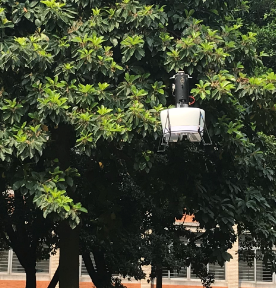
\includegraphics[scale=1]{Fig/DFUAV_f31.png} 
	% 添加标签one_DFUAV以及图标题“涵道风扇式无人机”,标题编号是自动生成的
	\caption{\label{one_DFUAV}涵道风扇式无人机} 
\end{figure}
\end{lstlisting}
其中figure为环境名,[htbp]表示将图片设置为浮动体,实际上这在.cls文件已经设置过,因而可以省略。[scale=1]表示安装1:1的比例导入图片,还可以按其他方式导入,需要时可自行百度。
\begin{figure}[htbp]
	\centering
	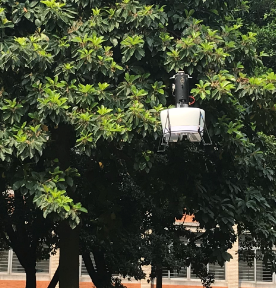
\includegraphics[scale=1]{Fig/DFUAV_f31.png}
	\caption{\label{one_DFUAV}涵道风扇式无人机}
\end{figure}

使用如下代码划分页面并排放置图\ref{Hawk}、图\ref{GTSpy}
\begin{lstlisting}
\begin{figure}[htbp]
	\centering
	\begin{minipage}[c]{0.5\textwidth} % minipage将页面划分为0.5\textwidth
		\centering
		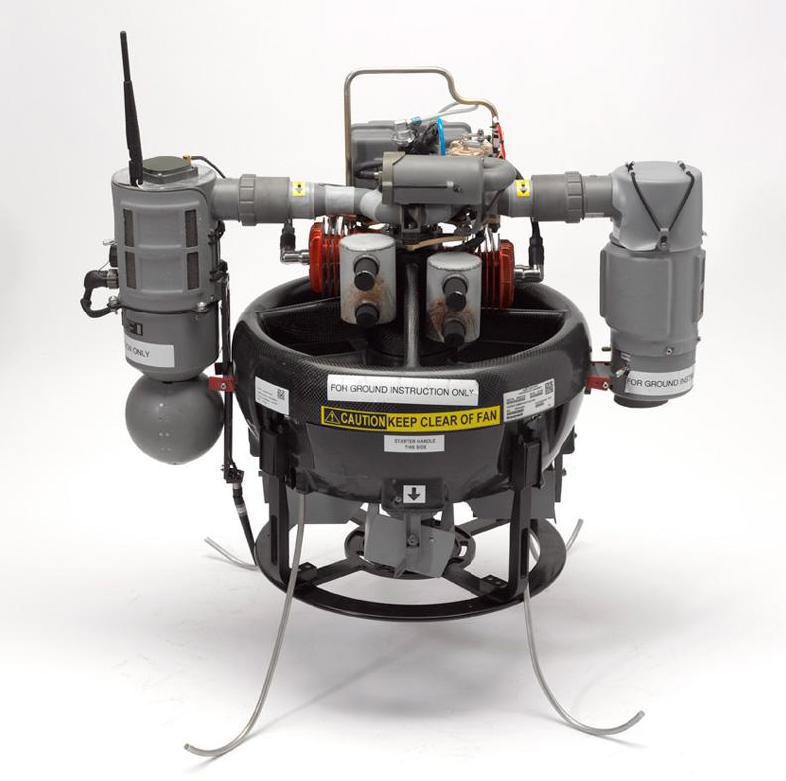
\includegraphics[width=6cm,height=6cm]{Fig/honeywell_t-hawk.jpg}
		\caption{\label{Hawk}T-Hawk}
	\end{minipage}%
	\begin{minipage}[c]{0.5\textwidth}
		\centering
		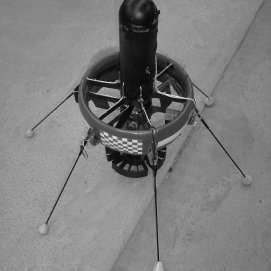
\includegraphics[width=6cm,height=6cm]{Fig/GTSpy.jpg}
		\caption{\label{GTSpy}GTSpy}
	\end{minipage}
\end{figure}
\end{lstlisting}
其中[c]表示行居中对齐。当图片大小不一但又需要1:1导入时,图标题可能行不对齐,因此可以改为如下指令:
\begin{lstlisting}
\begin{figure}[htbp]
	\centering
	\begin{minipage}[c]{0.5\textwidth}
		\centering
		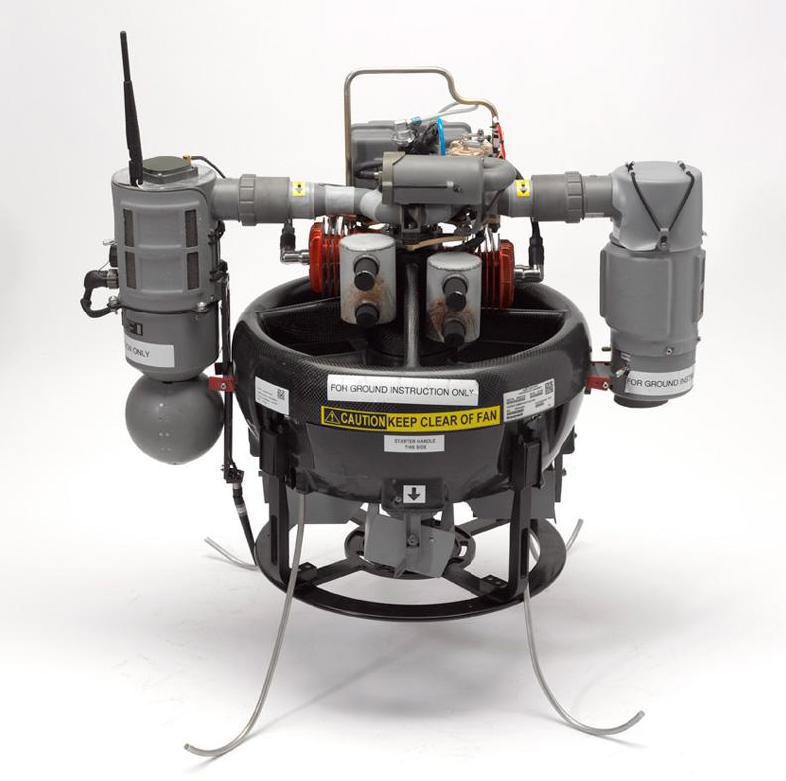
\includegraphics[scale=1]{Fig/honeywell_t-hawk.jpg} %1:1导入
	\end{minipage}%
	\begin{minipage}[c]{0.5\textwidth}
		\centering
		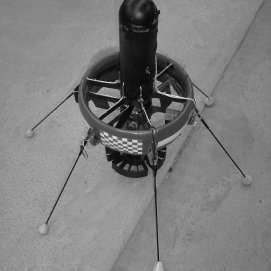
\includegraphics[scale=1]{Fig/GTSpy.jpg}
	\end{minipage}\\[1pt]
	\begin{minipage}[t]{0.5\textwidth}	% 以下为新添加页面划分,[t]表示行顶部对齐
		\caption{\label{Hawk}T-Hawk}
	\end{minipage}%
	\begin{minipage}[t]{0.5\textwidth}
		\caption{\label{GTSpy}GTSpy}
	\end{minipage}%
\end{figure}
\end{lstlisting}
\begin{figure}[htbp]
	\centering
	\begin{minipage}[c]{0.5\textwidth}
		\centering
		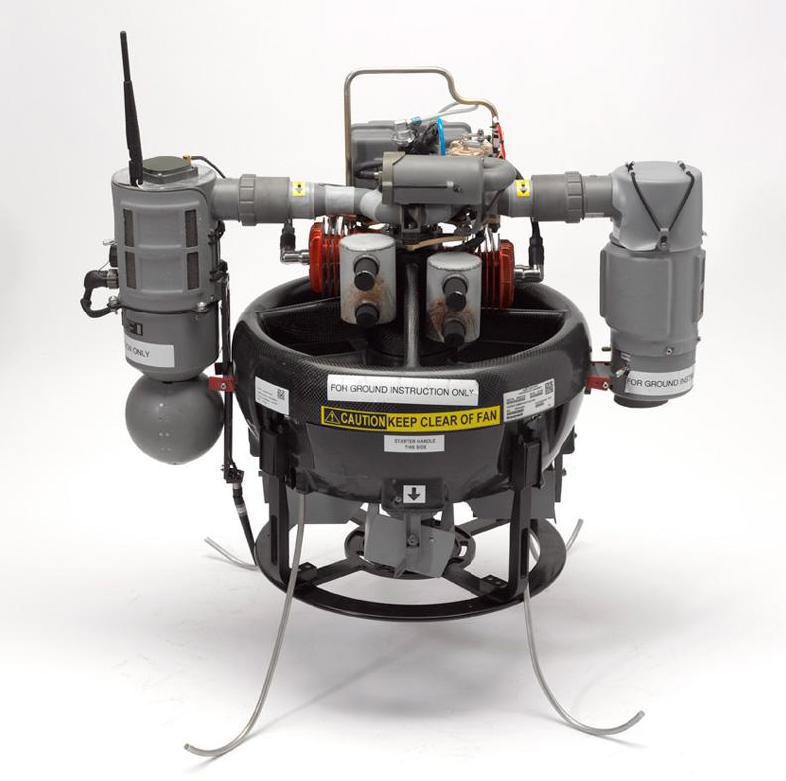
\includegraphics[width=6cm,height=6cm]{Fig/honeywell_t-hawk.jpg}
		\caption{\label{Hawk}T-Hawk}
	\end{minipage}%
	\begin{minipage}[c]{0.5\textwidth}
		\centering
		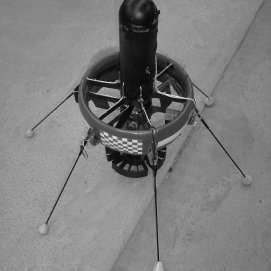
\includegraphics[width=6cm,height=6cm]{Fig/GTSpy.jpg}
		\caption{\label{GTSpy}GTSpy}
	\end{minipage}
\end{figure}
\section{表}
本节仅展示使用常见的三线表
\begin{lstlisting}
\begin{table}
	\caption{\label{TDF_para}涵道模型参数}	%表题在上
	\centering	% 表居中
	\small	% 表内字体小一号(即设置成和表题字号一致)
	\begin{tabular}{cccc}	% cccc表示4列并居中,若列之间需要分隔符则设置为|c|c|c|c|
		\hline	% \hline表示横线。列之间的元素用&分隔,\tabularnewline表示换行
		参数符号 & 数值 & 参数符号 & 数值 \tabularnewline 
		\hline 
		$I_x$ & $054593$ 		   & $I_y$ & $0.017045         $ \tabularnewline
		$l_1$ & $0.0808\,\text{m}$ & $l_2$ & $0.175\,\text{m}  $ \tabularnewline 
		$l_4$ & $0.2415\,\text{m}$ & $l_5$ & $0.1085\,\text{m} $ \tabularnewline
		\hline 
	\end{tabular}
\end{table}
\end{lstlisting}
\begin{table}
	\caption{\label{TDF_para}涵道模型参数}
	\centering
	\small 
	\begin{tabular}{cccc}
		\hline 
		参数符号 & 数值                & 参数符号 & 数值                 \tabularnewline
		\hline 
		$I_x$   & $054593$ 		     & $I_y$   & $0.017045         $ \tabularnewline
		$l_1$   & $0.0808\,\text{m}$ & $l_2$   & $0.175\,\text{m}  $ \tabularnewline 
		$l_4$   & $0.2415\,\text{m}$ & $l_5$   & $0.1085\,\text{m} $ \tabularnewline
		\hline 
	\end{tabular}
\end{table}
\added{表格的中英文题注,可以使用TableBicaption命令,与图片的用法一致}。
\section{公式}
除了前面讲行内公式,常用的还有行间公式。公式中的数学符号可自行百度,本章仅介绍常用的几种公式环境。

单独成行的行间公式在 \LaTeX{} 里由equation 环境包裹。equation 环境为公式自动生成一个编号,这个编号可以用\textbackslash{}label 和\textbackslash{}ref 生成交叉引用,amsmath 宏包的\textbackslash{}eqref 可为引用自动加上圆括号;如式\eqref{eq_1}所示。
\begin{lstlisting}
\begin{equation}
	a+b=c	\label{eq_1}
\end{equation}
\end{lstlisting}
\begin{equation}
	a+b=c	\label{eq_1}
\end{equation}
若不需要编号则加星号,改为
\begin{lstlisting}
\begin{equation*}
	a+b=c
\end{equation*}
\end{lstlisting}
其他环境类似。当使用 \texttt\$ 开启行内公式输入,或是使用{equation} 环境时,\LaTeX\ 就进入了数学模式。
数学模式相比于文本模式有以下特点:
\begin{enumerate}
	\item 数学模式中输入的空格被忽略。数学符号的间距默认由符号的性质(关系符号、运算符等)决定。
	需要人为引入间距时,使用 \textbackslash{}{quad} 和 \textbackslash{}{qquad} 等命令。
	\item {不允许有空行(分段)}。行间公式中也无法用 $ \verb|\\|$命令手动换行。排版多行公式需要用到 其他各种环境。
	\item 所有的字母被当作数学公式中的变量处理,字母间距与文本模式不一致,也无法生成单词之间的空格。
	如果想在数学公式中输入正体的文本,简单情况下可用 \textbackslash{}{mathrm} 命令。
	或者用 {amsmath} 提供的 \textbackslash{}{text} 命令(仅适合在公式中穿插少量文字。如果你的情况正好相反,需要在许多文字中穿插使用公式,则应该像正常的行内公式那样用,而不是滥用 \textbackslash{}{text} 命令)。
\end{enumerate}	

实际上更常用的的是多行公式,不需要对齐的公式组可以使用gather环境,需要对齐的公式组用align 环境。
长公式内可用$ \verb|\\|$ 换行。

如果需要罗列一系列公式,并令其按照等号对齐,可用align 环境,它将公式用\& 隔为两部分并对齐。分隔符通常放在等号左边:
\begin{lstlisting}
\begin{align}
	a & = b + c \\
	& = d + e
\end{align}
\end{lstlisting}
\begin{align}
a & = b + c \\
& = d + e
\end{align}
align 环境会给每行公式都编号。

如果不需要按等号对齐,只需罗列数个公式,可用gather环境:
\begin{lstlisting}
\begin{gather}
	a  = b + c \notag \\
	f = d + e 
\end{gather}
\end{lstlisting}
\begin{gather}
	a  = b + c \notag  \\
	f = d + e 
\end{gather}
gather 环境同样会给每行公式都编号,如果某行不需要编号可在行末用\textbackslash{}notag 仅去掉某行的编号。

align 和gather 有对应的不带编号的版本align* 和gather*。

另一个常见的需求是将多个公式组在一起公用一个编号,编号位于公式的居中位置。为此,
amsmath 宏包提供了诸如aligned、gathered 等环境,与equation 环境套用。以-ed 结尾的
环境用法与前一节不以-ed 结尾的环境用法一一对应。我们仅以aligned 举例:
\begin{lstlisting}
\begin{equation}
	\begin{aligned}
		a &= b + c \\
		d &= e + f + g \\
		h + i &= j + k \\
		l + m &= n
	\end{aligned}
\end{equation}
\end{lstlisting}
\begin{equation}
	\begin{aligned}
		a &= b + c \\
		d &= e + f + g \\
		h + i &= j + k \\
		l + m &= n
	\end{aligned}
\end{equation}
split 环境和aligned 环境用法类似,也用于和equation 环境套用,区别是split 只能
将每行的一个公式分两栏,aligned 允许每行多个公式多栏。

分段函数通常用amsmath 宏包提供的cases 环境,可参考文献\parencite{_c}

amsmath 宏包还直接提供了多种排版矩阵的环境,包括不带定界符的matrix,以及带各种定界符的矩阵pmatrix、bmatrix、Bmatrix、vmatrix、Vmatrix。
其中中括号版的bmatrix最常用。这些矩阵环境需要在公式中使用,比如 align 环境。
\begin{lstlisting}
A= \begin{bmatrix}
		x_{11} & x_{12} & \ldots & x_{1n} \\
		x_{21} & x_{22} & \ldots & x_{2n} \\
		\vdots & \vdots & \ddots & \vdots \\
		x_{n1} & x_{n2} & \ldots & x_{nn}
	\end{bmatrix}
\end{gather}
\end{lstlisting}
\begin{gather}
\bm{A}= \begin{bmatrix}
	x_{11} & x_{12} & \ldots & x_{1n} \\
	x_{21} & x_{22} & \ldots & x_{2n} \\
	\vdots & \vdots & \ddots & \vdots \\
	x_{n1} & x_{n2} & \ldots & x_{nn}
   \end{bmatrix}
\end{gather}	
其中矩阵/向量加粗使用\textbackslash{}bm\{\}命令。另外还可以使用array环境排版矩阵,类似tabular环境,用$ \verb|\\|$ 和\& 用来分隔行和列,这里不再赘述。	
\begin{lstlisting}
\begin{array }[外部对齐tcb]{列对齐lcr}
	行列内容
\end{array}
\end{lstlisting}

另外注意排版分式时,有两种方法:\textbackslash{}frac或者\textbackslash{}dfrac,效果分别为$ \frac{1}{2} $和$ \dfrac{1}{2} $。以上介绍的数学环境中,空格可参考文献\parencite{_c},例如常用\textbackslash{}quad。
\section{定理}
在scutthesis.cls文件536行开始,已经用\textbackslash{}newtheorem命令定义了几种定理环境,包括:定义、假设、定理、结论、引理、公理、推论、性质等等,统称定理环境,关于\textbackslash{}newtheorem的用法,可参考\cite{_c}或自行百度。要下面提供几个例子,在横线之间的深色区域是代码,效果在相应下方表示:
\begin{lstlisting}
\begin{assumption}
	加权矩阵${{\bm{W}}_{1}}$和 ${{\bm{W}}_{2}}$ 是对称矩阵,且$ {{\bm{W}}_{2}}$非奇异。	\label{assum_dca1}
\end{assumption}
\end{lstlisting}
\begin{assumption}
	加权矩阵${{\bm{W}}_{1}}$和 ${{\bm{W}}_{2}}$ 是对称矩阵,且$ {{\bm{W}}_{2}}$非奇异。	\label{assum_dca1}
\end{assumption}

定理用法和假设类似:
\begin{lstlisting}
\begin{theorem}
	如果假设\ref{assum_dca1}成立,$\bm{F}$满足式\eqref{eq_F}的定义,且${{\bm{W}}_{1}}$非奇异,则有$0\le e \left( \bm{F} \right) < 1$,其中$e \left( \bm{F} \right)$是 $\bm{F}$的特征值。	\label{the_dca2}
\end{theorem}
\end{lstlisting}
\begin{theorem}
	如果假设\ref{assum_dca1}成立,$\bm{F}$满足上式的定义,且${{\bm{W}}_{1}}$非奇异,则有$0\le e \left( \bm{F} \right) < 1$,其中$e \left( \bm{F} \right)$是 $\bm{F}$的特征值。	\label{the_dca2}
\end{theorem}

定理环境的编号可自定义,但通常不需要再进行设置,因为模板文件scutthesis.cls文件已经定义好。
\section{参考文献}

\begin{lstlisting}
关于参考文献这块,很多同学有疑问。只有记住一点:不管用什么参考文献管理工具,最终目的是生成一个bib文件给TeXstudio使用,bib文件里是特定格式的文献信息。bib文件可以使用一个叫notepad++的软件打开。
\end{lstlisting}

通常学位论文参考文献是基于BibTeX进行的,本模板最大的改进就是引入BibLaTeX。关于这部分知识可参考文献\cite{_c}的第六章,6.1节参考文献和BIBTEX工具。

参考文献引用和著录是基于ZOTERO这个软件进行的。视频教程见\parencite{_e}。此外,为了符合毕业论文撰写规范,需设置参数。按照视频教程安装完必要的插件(如Better BibTeX)后,在编辑->首选项进行设置。附录图\ref{op1}到图\ref{op11}所示的是我的zotero软件设置。其中最重要的是\ref{op10}的设置要排除的选项,多余的显示会让审稿人反感,按照论文撰写规范进行即可。在毕业论文撰写时,在编辑->首选项->Better BibLTeX->Fields中,Fields to omit from export填month,abstract,note,extra,file,keywords,type,url,doi,就是在参考文献著录中排除这些多余的项,避免过于复杂。而在写本模板使用说明时,没有排除url,因为很多参考资料是网页。

\begin{lstlisting}
使用zotero,科学上网很重要,通常我们使用谷歌学术搜索文献并利用chrome的zotero插件直接捕获文献著录信息。但我使用蓝灯,代理服务器均遇到过被谷歌学术封锁的情况。只能不断换科学上网方法。这里我现在用的chrome插件:谷歌上网助手,它可以轻松捕获谷歌学术的著录信息,注册一个账号即可使用。谷歌上网助手有可能和某些代理冲突。这些都是科学上网的问题,已经超出了本项目的范围,听说百度一下 v2ray 可发现新大陆,可惜我试了Vultr的服务器依然被谷歌封。知网捕获中文参考文献著录信息的话不需要考虑这个问题,直接在知网首页搜索文献然后点击插件既可以选想捕获的著录了。
\end{lstlisting}

在zotero软件点击文件->导出文献库,如图\ref{output}所示,再在导出对话框图\ref{output_format}选择导出格式为Better BibLaTeX,同时勾选Keep updated选项保持自动更新,再点击ok,在弹出的对话框图\ref{output_name}确定保存路径和文件名,例如我的是MyLibrary.bib,这也是我整个读书生涯的文献库bib文件。如果写小论文的话通常导出格式是BibTeX或者Better BibTeX(这里按照期刊的要求来即可,文献管理软件的好处就是快速自动生成一个文件库)。关于BibTeX和BibLaTeX的区别这里不做展开。

得到文献库后,在scutthesis.tex文件第九行使用\textbackslash{}addbibresource命令,添加文献库。引用某文献时秩序在zotero选中某文献条目,然后按Ctrl+Shift+C,复制引用关键字(Citation Key)到剪切板(快捷键可自定义)。然后在tex文件编辑界面直接粘贴,默认的时上标形式,若需要非上标形式,可以改为\textbackslash{}parencite{XXXX},其中XXXX是Citation Key。这里的操作和认为设置的首选项参数有关,需要在编辑->首选项->导出界面的默认格式一栏选中相应的项,同时在编辑->首选项->高级->快捷键设置为默认值。

---------------------------------------------------------------------------------

2020年12月2日测试:
下载最新zotero,从知网和谷歌捕获文献(刚打开网页最好稍等一会再点击插件,谷歌可能需要现人机验证),对文献\parencite{Renduchintala_2019}、\parencite{Meng_2020}进行引用。

---------------------------------------------------------------------------------
\begin{lstlisting}
另外有同学反映,换了电脑后重新导出的bib文件Citation Key值不同,记得设置好Better BibTeX之后,在著录条目界面全选著录(或仅选想更新的著录)然后右键选Better BibTeX更新refresh一下。然后在Automatic export选项点击Export now立即更新bib文件(按理说勾选了自动更新选项他会自动更新,但为了确保万无一失还是点一下)。
\end{lstlisting}










%第三章
	\chapter{一些修改之处——By CYX}
2022年学校更新了双盲评审的要求与规范,同时,本人在使用祖传模版过程中,也遇到了一些问题,对前辈们的模版进行了一些细节修改,本章主要介绍本人对祖传模版的更改。

\section{双盲评审}
双盲评审论文要求隐去作者及导师信息,因此论文封面及成果列表需要进行变更,且论文构成中,盲审论文不包括致谢部分。

导言区option控制论文封面,mainManuscript.tex文末部分代码控制成果列表及致谢。
\begin{lstlisting}
    \ifpdfcover
        \ifreview
            \chapter{攻读博士学位期间取得的研究成果}

一、已发表(包括已接受待发表)的论文,以及已投稿、或已成文打算投稿、或拟成文投稿的论文情况\underline{\textbf{(只填写与学位论文内容相关的部分):}}

\begin{centering}
	\small
	\begin{longtable}{|>{\centering}m{0.5cm}|>{\centering}m{5.5cm}|>{\centering}m{2.7cm}|>{\centering}m{1.8cm}|>{\centering}m{1.8cm}|>{\centering}m{1cm}|}
		\hline 
		\textbf{序号}  & \textbf{发表或投稿刊物名称、级别}& \textbf{作者(仅注明第几作者)} & \textbf{发表年份} & \textbf{与学位论文哪一部分(章、节)相关} & \textbf{被索引收录情况}\tabularnewline
		\hline 
		1   & Journal of Manufacturing Processes\\(IF:5.01, JCR Q2) & 第一作者 &2021 & 第五章 & SCI\tabularnewline
		\hline 
		2	& 可继续往下添加 &第一作者& 2021& 第四章 & SCI \tabularnewline
		\hline
	\end{longtable}
\end{centering}

二、与学位内容相关的其它成果(包括专利、著作、获奖项目等)

1、与学位内容相关的著作

参与编写一本著作,导师第一、学生第二,2021,与学位论文第三章、第六章相关

2、与学位内容相关的专利

已授权一项发明专利,导师第一、学生第二,2021,与学位论文第二章、第四章和第五章相关

已受理一项发明专利,导师第一、学生第三,2020,与学位论文第二章相关

已授权一项发明专利,导师第一、学生第五,2018,与学位论文第二章相关

已授权一项软件著作权,导师第一、学生第三,2020,与学位论文第二章相关
 %成果-盲审版
        \else
            \chapter{攻读博士学位期间取得的研究成果}

一、已发表(包括已接受待发表)的论文,以及已投稿、或已成文打算投稿、或拟成文投稿的论文情况\underline{\textbf{(只填写与学位论文内容相关的部分):}}

\begin{centering}
	\small
	\begin{longtable}{|>{\centering}m{0.5cm}|>{\centering}m{2.2cm}|>{\centering}m{3.3cm}|>{\centering}m{2.7cm}|>{\centering}m{1.8cm}|>{\centering}m{1.8cm}|>{\centering}m{1cm}|}
		\hline 
		\textbf{序号} & \textbf{作者} & \textbf{题\qquad 目} 						   & \textbf{发表或投稿刊物名称、级别} & \textbf{发表的卷期、年月、页码} & \textbf{与学位论文哪一部分(章、节)相关} & \textbf{被索引收录情况}\tabularnewline
		\hline 
		1   & \textbf{Cui Yanxin}, Kang Youping,\\ Shi Yonghua, Chen Jinrong, Wang Zishun, Wang Jinyi & Investigation into the arc profiles and penetration ability of axial magnetic field-enhanced K-TIG welding by means of a specially designed sandwich & Journal of Manufacturing Processes\\(IF:5.01, JCR Q2) & 2021, 68:32-41 & 第五章 & SCI\tabularnewline
		\hline 
		2	& \textbf{Cui Yanxin}, Shi Yonghua, Hong Xiaobin & To be continued & Journal of Manufacturing Processes\\(IF:5.01, JCR Q2)  & 2019, 46:225-233 & 第六章 &SCI \tabularnewline
		\hline
	\end{longtable}
\end{centering}
\newpage
二、与学位内容相关的其它成果(包括专利、著作、获奖项目等)

1、与学位内容相关的著作

\begin{centering}
	\small
	\begin{longtable}{|>{\centering}m{0.5cm}|>{\centering}m{2.2cm}|>{\centering}m{4.7cm}|>{\centering}m{2.7cm}|>{\centering}m{1.8cm}|>{\centering}m{1.8cm}|}
		\hline 
		\textbf{序号} & \textbf{作者} & \textbf{著作名称} 						   & \textbf{出版社} & \textbf{出版的年月、页码} & \textbf{与学位论文哪一部分(章、节)相关} \tabularnewline
		\hline 
		1	& Shi Yonghua, \textbf{Cui Yanxin}, Cui Shuwan, Zhang Baori & A Novel High-Efficiency Keyhole Tungsten Inert Gas (K-TIG) Welding: Principles and Practices & Welding Technology. Cham: Springer International Publishing & 2021: 313–367 & 第三章\\第六章\tabularnewline
		\hline
	\end{longtable}
\end{centering}

2、与学位内容相关的专利

\begin{centering}
	\small
	\begin{longtable}{|>{\centering}m{0.5cm}|>{\centering}m{4cm}|>{\centering}m{3.5cm}|>{\centering}m{4cm}|>{\centering}m{2.2cm}|}
		\hline
		\textbf{序号}	&	\textbf{专利申请人}	&	\textbf{专利名称}	&	\textbf{专利号}	&	\textbf{与学位论文哪一部分(章、节)相关}\tabularnewline
		\hline
		1	& 石永华,\textbf{崔延鑫},陈金荣,陈云可	&	一种用于锁孔效应深熔TIG焊的电弧压力测量装置与方法	&	发明专利202110489846.6(已授权)	& 第二章\tabularnewline
		\hline
		2	& ***	& 	***	& ***	& 第二章\tabularnewline
		\hline
	\end{longtable}
\end{centering} %成果-最终版
            \chapter{致\texorpdfstring{\quad}{}谢}
%把下面文字替换
感谢各位前辈提供的模版!

%把上面文字替换

~\\

\begin{minipage}[t]{0.945\textwidth}%
	\begin{flushright}
		崔延鑫\\
		\today\\	% 自动时间
		%2022年4月6日\\	%固定时间
		于华南理工大学
		\par\end{flushright}
\end{minipage}

 %致谢
        \fi
    \fi
\end{lstlisting}
\subsection{论文封面}
使用时,现在对应的wrod文件中修改封面信息,导出为对应的review\_cover.pdf或thesis\_cover.pdf,通过控制导言区文档类option选择采用哪种封面。
\begin{lstlisting}
    \documentclass[unicode,master,pdfcover]{scutthesis}	% 使用pdf文件封面的最终版硕士学位论文模板
    \documentclass[unicode,master]{scutthesis}	% 不使用pdf文件封面的 硕士模板
    \documentclass[unicode,pdfcover]{scutthesis}	% 使用pdf文件封面的最终版博士学位论文模板
    \documentclass[unicode]{scutthesis}	% 不使用pdf文件封面的博士模板,即草稿封面
    \documentclass[unicode,pdfcover,review]{scutthesis}	% 使用pdf文件封面的送审版的博士学位论文模版
\end{lstlisting}
\subsection{成果列表}
成果列表中,根据学校的格式,设计了pub.tex或pub-review.tex中的表格格式,注意使用\textbackslash{}tabularnewline命令换行,表内换行可以使用\textbackslash{}\textbackslash{}。

表格命令如下,在使用时,可以微调\{**cm\}的距离,不过,本人已在Adobe Illustrator中核对了表格每栏的距离,目前这个距离恰好,若有需要,可自行变更调整距离。
\begin{lstlisting}
    \begin{centering}
        \small
        \begin{longtable}{|>{\centering}m{0.5cm}|>{\centering}m{5.5cm}|>{\centering}m{2.7cm}|>{\centering}m{1.8cm}|>{\centering}m{1.8cm}|>{\centering}m{1cm}|}
            \hline 
            \textbf{序号}  & \textbf{发表或投稿刊物名称、级别}& \textbf{作者(仅注明第几作者)} & \textbf{发表年份} & \textbf{与学位论文哪一部分(章、节)相关} & \textbf{被索引收录情况}\tabularnewline
            \hline 
            1   & Journal of Manufacturing Processes\\(IF:5.01, JCR Q2) & 第一作者 &2021 & 第五章 & SCI\tabularnewline
            \hline 
            2	& 可继续往下添加 &第一作者& 2021& 第四章 & SCI \tabularnewline
            \hline
        \end{longtable}
    \end{centering}
\end{lstlisting}

\section{浮动体相关}
\subsection{中英文题注}
对于博士学位论文,需要中英文题注,可以使用如下代码,效果如图\ref{one_DFUAV_2}。图片与表格的中英文题注分别使用的命令为\textbackslash{}FigureBicaption\{\}\{\}与\textbackslash{}TableBicaption\{\}\{\}。
\begin{lstlisting}
    \begin{figure}[htbp]
        % 图片居中(列居中对齐)
        \centering	
        % 包含当前路径下的Fig文件夹的图片文件DFUAV_f31.png
        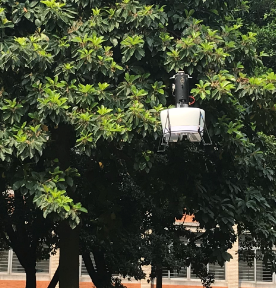
\includegraphics[scale=1]{Fig/DFUAV_f31.png} 
        % 添加标签one_DFUAV以及图标题“涵道风扇式无人机”,标题编号是自动生成的
        \FigureBicaption{\label{one_DFUAV_2}涵道风扇式无人机}{The English caption} 
    \end{figure}
\end{lstlisting}
\begin{figure}[htbp]
    % 图片居中(列居中对齐)
    \centering	
    % 包含当前路径下的Fig文件夹的图片文件DFUAV_f31.png
    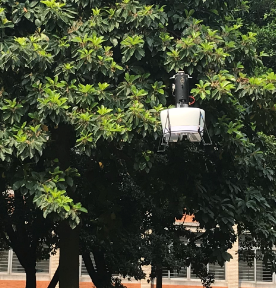
\includegraphics[scale=1]{Fig/DFUAV_f31.png} 
    % 添加标签one_DFUAV以及图标题“涵道风扇式无人机”,标题编号是自动生成的
    \FigureBicaption{\label{one_DFUAV_2}涵道风扇式无人机}{The English caption} 
\end{figure}

值得说明的是,本人修改了cls模版中题注与表格、图片的距离。华工官方提供的格式说明中并未提及中英文题注的行距要求,本人根据上交与清华的博士学位论文格式规范,与几位老师沟通后,修改了题注的行距,具体表现为:
\begin{enumerate}
    \item 中英文题注间保持正文行距,即1.5倍行距。
    \item 中文题注段前\qty{4}{\pt},图片环境下,段后\qty{-8}{\pt};表格环境下,段后\qty{0}{\pt}。
    \item 单独的中或英题注,当文字过长时,应为单倍行距,此处改动暂未实现。(Todo)
\end{enumerate}

若要改动中英文题注间距,可在cls模版对应命令处更改,如下。
\begin{lstlisting}
\newcommand{\FigureBicaption}[2]{
  \renewcommand{\figurename}{图}
  \vspace{4pt} %段前
  \caption{#1}
  \addtocounter{figure}{-1}
  \renewcommand{\figurename}{Fig.}
  \captionsetup{list=false}
  %\vspace{3pt} %中文与英文题注间行距,此行注释掉即保持与正文一致的1.5倍行距。
  \caption{#2}
  \captionsetup{list=true}
  \renewcommand{\figurename}{图}
  \vspace{-8pt} %英文题注段后间距,因float环境默认了一定的间距,经多次尝试后定为-8pt较为美观
}
\end{lstlisting}
\begin{lstlisting}
\newcommand{\TableBicaption}[2]{
  \renewcommand{\tablename}{表}
  \vspace{4pt} %段前
  \caption{#1}
  %\vspace{3pt} %中文与英文题注间行距,此行注释掉即保持与正文一致的1.5倍行距。
  \addtocounter{table}{-1}
  \renewcommand{\tablename}{Table}
  \captionsetup{list=false}
  \caption{#2}
  \captionsetup{list=true}
  \renewcommand{\tablename}{表}
  %\vspace{-2pt} %英文题注段后间距,因表格题注后紧跟表格内容,经试验,此行注释掉较为美观
}
\end{lstlisting}

值得说明的是,原模版对于题注的字号设置为\qty{10.95}{\pt},然而,五号字体应改为\qty{10.5}{\pt},原设置会让题注字号较大。

原模版英文题注比较长时,第二行的题注不再居中,为此,本人修改了figure与table的caption设置,如下:
\begin{lstlisting}
    \captionsetup[figure]{position=bottom,justification=centering}
    \captionsetup[table]{position=top,justification=centering}
\end{lstlisting}
\subsection{超宽图片处理}
有时,个别图片会超出文本区域范围,在原模版文件中,超宽图片左侧边栏默认与文本区域左侧进行左对齐,因此,图片会不在居中位置。为解决这个问题,在图片浮动体命令中,使用下述命令替换\textbackslash{}centering。
\begin{lstlisting}
\setlength{\leftskip}{0pt plus 1fil minus \marginparwidth}
\setlength{\rightskip}{\leftskip}
\end{lstlisting}
\subsection{超宽三线表处理}
有时,三线表结构比较简单,如表\ref{tab:chapter6_featureNumber}所示,表头只有序号与特征,若竖排,会占据非常多的空间,将其转换到横排,需要按照
《CY/T 170—2019学术出版规范表格》,使用双竖细线分隔重复的表头。
\begin{table}[htb]
    \setlength{\belowrulesep}{0pt}
    \setlength{\aboverulesep}{0pt}
    \setlength\arrayrulewidth{0.6pt}
    \centering
    \TableBicaption{特征编号}{The feature number}\label{tab:chapter6_featureNumber}
    \wuhao
    \begin{tabular}{cc||cc||cc}
    \toprule
    序号    &   特征    &   序号    &   特征    &   序号    &   特征\\
    \hhline{--||--||--}
    1   &   $D_1$   &    8    &   $f_5$      &   15    &  $MFCC 6$     \\
    2   &   $R_1$   &    9    &   $E$        &   16    &  $MFCC 7$     \\
    3   &   $K_1$   &    10   &   $MFCC 1$   &   17    &  $MFCC 8$     \\
    4   &   $R_2$   &    11   &   $MFCC 2$   &   18    &  $MFCC 9$     \\
    5   &   $K_2$   &    12   &   $MFCC 3$   &   19    &  $MFCC 10$     \\
    6   &   $f_2$   &    13   &   $MFCC 4$   &   -     &    -   \\
    7   &   $f_4$   &    14   &   $MFCC 5$   &   -     &    -   \\
    \bottomrule
    \end{tabular}
\end{table}

基于这个目的,在导言区外加了makecell与hhline宏包,进行表格的设置,表\ref{tab:chapter6_featureNumber}代码如下:
\begin{lstlisting}
    \begin{table}[htb]
        \setlength{\belowrulesep}{0pt}
        \setlength{\aboverulesep}{0pt}
        \setlength\arrayrulewidth{0.6pt}
        \centering
        \TableBicaption{特征编号}{The feature number}\label{tab:chapter6_featureNumber}
        \wuhao
        \begin{tabular}{cc||cc||cc}
        \toprule
        序号    &   特征    &   序号    &   特征    &   序号    &   特征\\
        \hhline{--||--||--}
        1   &   $D_1$   &    8    &   $f_5$      &   15    &  $MFCC 6$     \\
        2   &   $R_1$   &    9    &   $E$        &   16    &  $MFCC 7$     \\
        3   &   $K_1$   &    10   &   $MFCC 1$   &   17    &  $MFCC 8$     \\
        4   &   $R_2$   &    11   &   $MFCC 2$   &   18    &  $MFCC 9$     \\
        5   &   $K_2$   &    12   &   $MFCC 3$   &   19    &  $MFCC 10$     \\
        6   &   $f_2$   &    13   &   $MFCC 4$   &   -     &    -   \\
        7   &   $f_4$   &    14   &   $MFCC 5$   &   -     &    -   \\
        \bottomrule
        \end{tabular}
    \end{table}
\end{lstlisting}

\section{公式及物理量}
在华工的学位论文要求中,明确了公式及物理量等部分应使用Times New Roman字体,尽管\LaTeX{}默认的字体更为美观。因此,本人修改了cls模版中公式字体设置,并使用siuntix宏包进行物理量的输入。
\subsection{公式环境字体}
尽管原模版中使用了如下代码,但公式及siuntix宏包涉及的物理量仍为默认字体,因此,需要对cls模版进行更改以满足格式要求。
\begin{lstlisting}
    \setmainfont[Mapping=tex-text]{Times New Roman}%\rmfamily 使用的字体,默认英文和数字的字体。
\end{lstlisting}

本文使用mathastext与mathspec宏包更改公式环境字体,在cls模版中,代码如下,注意amsmath宏包一定要在fontspec宏包前声明,fontspec宏包需有no-math的option,最后声明mathspec。
\begin{lstlisting}
    %% 为了实现公式字体为Times New Roman
    \RequirePackage{amsmath}
    \RequirePackage[no-math]{fontspec}
    \RequirePackage{mathspec}
\end{lstlisting}
在正文中,代码如下,需注意,italic选项意在指定公式环境为斜体的Times New Roman。
\begin{lstlisting}
    \usepackage[italic,defaultmathsizes]{mathastext}
\end{lstlisting}
\subsection{物理量}
物理量的格式有两个要求,分别是:
\begin{enumerate}
    \item 物理量本身字体应为Times New Roman。
    \item 物理量中,数字与单位之间应间隔$1/6m$的间距。
\end{enumerate}

本文使用siuntix宏包进行物理量输入,在正文中代码为:
\begin{lstlisting}
\usepackage{siunitx}
\sisetup{input-digits = 0123456789\pi}
\sisetup{per-mode = symbol}%
\DeclareSIUnit \vHardness {Hv} % 维氏硬度Hv
\DeclareSIUnit \dBA {dBA} % 动态范围
\DeclareSIUnit \mT {mT} % 特斯拉
\DeclareSIUnit \pt {pt} % pt
\newcommand{\qtyRange}[3]{\qtyrange[range-units=single,range-phrase=-]{#1}{#2}{#3}} % 单位范围
\newcommand{\numRange}[2]{\numrange[range-phrase=-]{#1}{#2}}	% 数字范围
\end{lstlisting}

本文自定义了输入数字或单位范围的命令,如数字范围命令为\textbackslash{}numRange\{\}\{\},例:\numRange{1}{10};单位范围命令为\textbackslash{}qtyRange\{\}\{\},例:\qtyRange{1}{10}{\mT}。更多
细节请查阅siuntix宏包官方文档。

\section{参考文献}
参考文献相关的修改主要有三个方面,一是连续两篇文献引用时的标注,二是参考文献列表的条目间行距,三是参考文献页末空白的修改。
\subsection{参考文献标注}
对于连续3个以上的参考文献,毫无疑问要标注为[1-3],然而,对于连续2个参考文献,目前大多数老师倾向于标注为[1,2],即\cite{_,_a}。尽管在最新的国标中,连续2个参考文献应标注为[1-2],但本人还是按照老师们的意见,修改了
gb7714-2015宏包对应的代码,使用[1,2]标注格式。相应文件为gb7714-2015.cbx,修改处如下,注意,cbx文件中有多个需要修改的地方,但都有“1改为0”的标注,全局搜索修改即可。
\begin{lstlisting}
%将连续3篇文献压缩改为连续2篇文献压缩
%
%该宏的目的是抛弃压缩内部的编号,而仅输出最后一个编号,主要通过cbx@tempcnta来控制
%一般情况下cbx@tempcnta为0,所以该宏不输出任何内容。当cbx@tempcnta在cite:comp:comp宏中更改变大后
%说明开始进入需要压缩的范围,当到压缩终点时,cbx@tempcnta必然大于1,则输出内容。
%修改第二行的数字1为0即可将默认的3个开始压缩变为2个开始压缩。
\renewbibmacro*{cite:dump}{%
  \ifnumgreater{\value{cbx@tempcnta}}{0}%
    {\ifnumgreater{\value{cbx@tempcnta}}{1}%1改为0,可以将压缩起始3个编号改为2个编号
       {\bibrangedash}%
       {\multicitedelim}%
     \bibhyperref[\cbx@lastkey]{%
       \ifdef\cbx@lastprefix%
         {\printtext[labelprefix]{\cbx@lastprefix}}%
         {}%
       \printtext[labelnumber]{\cbx@lastnumber}}}%
    {}%
  \setcounter{cbx@tempcnta}{0}%
  \global\undef\cbx@lastprefix}
\end{lstlisting}

值得说明的是,gb7714-2015宏包是随着TeXLive安装到电脑上的,最新版已默认标注格式为[1-2],若需要改为[1,2]则按上文说明进行更改,否则无需理会本节内容。
\subsection{参考文献列表条目行距}
原模版的参考文献列表中,条目间行距明显不是1.5倍行距。因此,在主文件中添加了下述语句,保证行距的一致性。
\begin{lstlisting}
\setlength{\bibitemsep}{0ex} % 设置参考文献条目间距离 revised by CYX
\end{lstlisting}
\subsection{参考文献跨页设置}
原始模版中,参考文献存在跨页的默认设置,导致页末(页尾上方)有时存在较大空行,因此,对参考文献进一步设置,取消了排版过大空行。
\begin{lstlisting}
    \renewcommand{\bibsetup}{
        \interlinepenalty=1000\relax
        \widowpenalty=1000\relax
        \clubpenalty=1000\relax
        \raggedbottom
    } % 参考文献条目跨页设置,避免太大空行 by CYX
\end{lstlisting}

\section{标题}
\subsection{单倍行距}
有时,标题的长度会比较长,一行无法全部写下,这时标题会发生换行,而在原模版文件中,全文默认1.5倍行距,因此,这种过长的标题格式会不符合规范,本模版对其进行了更改。由于笔者论文只涉及到了章节标题与各节一级标题的过长,
因此只修改了章节标题与一级标题的行距问题,若使用者有对其他标题格式修改的需要,只需自行添加\textbackslash{}linespread\{1\}命令。
\begin{lstlisting}
\newcommand{\textchapterfont}{\linespread{1}\centering\heiti\xiaoerhao} % 正文上第X章的字体 % 增添了章节标题单倍行距 ---By CYX
\newcommand{\textsectionfont}{\linespread{1}\heiti\xiaosanhao}            % 正文上X.Y节的字体 % 增添了一级标题单倍行距 ---By CYX
\end{lstlisting}
\subsection{三级标题格式}
三级标题应为小四号黑体,居左,原模版设置错误,笔者对其进行了修改。

\section{提交图书馆版}
提交图书馆时,需要末页附上答辩决议,版权页也需要签名,版权页更改可以在word中,对于答辩决议页,在tex文件中增添了下句:
\begin{lstlisting}
    \includepdf[pages=-]{decision.pdf} % 提交图书馆时使用 by CYX
\end{lstlisting}

平常这是注释掉的,最后提交时,将答辩决议保存为pdf文件,使用此句可以附在论文末页。
%第四章
	% 自行根据需要添加章节。

	\backmatter %章节不编号但页码继续
	%%%%%%%%%%%%%%%%%%%%%%%%%%%%%%%%%%%%%%%%%%%%%%%%%%%%%%%%%%%%%%    微调,使得后续章节的页眉不带章号——by MCH
	\renewcommand{\chaptermark}[1]{\markboth{#1}{}}
	%%%%%%%%%%%%%%%%%%%%%%%%%%%%%%%%%%%%%%%%%%%%%%%%%%%%%%%%%%%%%%
	\chapter{结\texorpdfstring{\quad}{}论}
本文主要是展示如何使用修改“祖传模板”得到的新模板,在使用时直接替换成自己的论文内容即可。总结下来最最最麻烦的是科学上网,只有科学上网才能获取文献信息生成bib文件,后面就好办了。

本模板难免有不足之处,主要是我本人的论文涉及的格式有限,有些地方没探索到自然就没去设置。比如附录,附录的图文并茂等等,我本人是没有研究的,这里仅仅做了一些初步的工作,不过对很多同学来说本模板是够用的。希望有能帮助到华工的同学们,有不足之处请多多理解,可以通过邮件联系我,上班之余我会尽量回复。 %结论
	 %%%%%%%%%%%%%%%%%%%%%%%%%%%%%%%%%%%%%%%%%%%%%% bibtex参考文献设置  (原版)
%%	\bibliographystyle{scutthesis}
%%	\bibliography{F:/MyLibrary}
	%%%%%%%%%%%%%%%%%%%%%%%%%%%%%%%%%%%%%%%%%%%%%%
	%%%%%%%%%%%%%%%%%%%%%%%%%%%%%%%%%%%%%%%%%%%%%% biber参考文献设置	——by MCH
	\addcontentsline{toc}{chapter}{参考文献}	%目录中添加参考文献
	\printbibliography	% 参考文献著录
 	%%%%%%%%%%%%%%%%%%%%%%%%%%%%%%%%%%%%%%%%%%%%%% ——by CYX
	\ifpdfcover
		\ifreview
			\chapter{攻读博士学位期间取得的研究成果}

一、已发表(包括已接受待发表)的论文,以及已投稿、或已成文打算投稿、或拟成文投稿的论文情况\underline{\textbf{(只填写与学位论文内容相关的部分):}}

\begin{centering}
	\small
	\begin{longtable}{|>{\centering}m{0.5cm}|>{\centering}m{5.5cm}|>{\centering}m{2.7cm}|>{\centering}m{1.8cm}|>{\centering}m{1.8cm}|>{\centering}m{1cm}|}
		\hline 
		\textbf{序号}  & \textbf{发表或投稿刊物名称、级别}& \textbf{作者(仅注明第几作者)} & \textbf{发表年份} & \textbf{与学位论文哪一部分(章、节)相关} & \textbf{被索引收录情况}\tabularnewline
		\hline 
		1   & Journal of Manufacturing Processes\\(IF:5.01, JCR Q2) & 第一作者 &2021 & 第五章 & SCI\tabularnewline
		\hline 
		2	& 可继续往下添加 &第一作者& 2021& 第四章 & SCI \tabularnewline
		\hline
	\end{longtable}
\end{centering}

二、与学位内容相关的其它成果(包括专利、著作、获奖项目等)

1、与学位内容相关的著作

参与编写一本著作,导师第一、学生第二,2021,与学位论文第三章、第六章相关

2、与学位内容相关的专利

已授权一项发明专利,导师第一、学生第二,2021,与学位论文第二章、第四章和第五章相关

已受理一项发明专利,导师第一、学生第三,2020,与学位论文第二章相关

已授权一项发明专利,导师第一、学生第五,2018,与学位论文第二章相关

已授权一项软件著作权,导师第一、学生第三,2020,与学位论文第二章相关
 %成果-盲审版
		\else
			\chapter{攻读博士学位期间取得的研究成果}

一、已发表(包括已接受待发表)的论文,以及已投稿、或已成文打算投稿、或拟成文投稿的论文情况\underline{\textbf{(只填写与学位论文内容相关的部分):}}

\begin{centering}
	\small
	\begin{longtable}{|>{\centering}m{0.5cm}|>{\centering}m{2.2cm}|>{\centering}m{3.3cm}|>{\centering}m{2.7cm}|>{\centering}m{1.8cm}|>{\centering}m{1.8cm}|>{\centering}m{1cm}|}
		\hline 
		\textbf{序号} & \textbf{作者} & \textbf{题\qquad 目} 						   & \textbf{发表或投稿刊物名称、级别} & \textbf{发表的卷期、年月、页码} & \textbf{与学位论文哪一部分(章、节)相关} & \textbf{被索引收录情况}\tabularnewline
		\hline 
		1   & \textbf{Cui Yanxin}, Kang Youping,\\ Shi Yonghua, Chen Jinrong, Wang Zishun, Wang Jinyi & Investigation into the arc profiles and penetration ability of axial magnetic field-enhanced K-TIG welding by means of a specially designed sandwich & Journal of Manufacturing Processes\\(IF:5.01, JCR Q2) & 2021, 68:32-41 & 第五章 & SCI\tabularnewline
		\hline 
		2	& \textbf{Cui Yanxin}, Shi Yonghua, Hong Xiaobin & To be continued & Journal of Manufacturing Processes\\(IF:5.01, JCR Q2)  & 2019, 46:225-233 & 第六章 &SCI \tabularnewline
		\hline
	\end{longtable}
\end{centering}
\newpage
二、与学位内容相关的其它成果(包括专利、著作、获奖项目等)

1、与学位内容相关的著作

\begin{centering}
	\small
	\begin{longtable}{|>{\centering}m{0.5cm}|>{\centering}m{2.2cm}|>{\centering}m{4.7cm}|>{\centering}m{2.7cm}|>{\centering}m{1.8cm}|>{\centering}m{1.8cm}|}
		\hline 
		\textbf{序号} & \textbf{作者} & \textbf{著作名称} 						   & \textbf{出版社} & \textbf{出版的年月、页码} & \textbf{与学位论文哪一部分(章、节)相关} \tabularnewline
		\hline 
		1	& Shi Yonghua, \textbf{Cui Yanxin}, Cui Shuwan, Zhang Baori & A Novel High-Efficiency Keyhole Tungsten Inert Gas (K-TIG) Welding: Principles and Practices & Welding Technology. Cham: Springer International Publishing & 2021: 313–367 & 第三章\\第六章\tabularnewline
		\hline
	\end{longtable}
\end{centering}

2、与学位内容相关的专利

\begin{centering}
	\small
	\begin{longtable}{|>{\centering}m{0.5cm}|>{\centering}m{4cm}|>{\centering}m{3.5cm}|>{\centering}m{4cm}|>{\centering}m{2.2cm}|}
		\hline
		\textbf{序号}	&	\textbf{专利申请人}	&	\textbf{专利名称}	&	\textbf{专利号}	&	\textbf{与学位论文哪一部分(章、节)相关}\tabularnewline
		\hline
		1	& 石永华,\textbf{崔延鑫},陈金荣,陈云可	&	一种用于锁孔效应深熔TIG焊的电弧压力测量装置与方法	&	发明专利202110489846.6(已授权)	& 第二章\tabularnewline
		\hline
		2	& ***	& 	***	& ***	& 第二章\tabularnewline
		\hline
	\end{longtable}
\end{centering} %成果-最终版
			\chapter{致\texorpdfstring{\quad}{}谢}
%把下面文字替换
感谢各位前辈提供的模版!

%把上面文字替换

~\\

\begin{minipage}[t]{0.945\textwidth}%
	\begin{flushright}
		崔延鑫\\
		\today\\	% 自动时间
		%2022年4月6日\\	%固定时间
		于华南理工大学
		\par\end{flushright}
\end{minipage}

 %致谢
		\fi
	\fi
	% \includepdf[pages=-]{decision.pdf} % 提交图书馆时使用 by CYX
\end{document}
